\documentclass[portrait,final,a0paper,fontscale=0.277]{baposter}

\usepackage[utf8]{inputenc}
\usepackage[spanish]{babel}
\usepackage{calc}
\usepackage{graphicx,amscd,calc}
\usepackage{amsmath}
\usepackage{amssymb}
\usepackage{relsize}
\usepackage{multirow}
\usepackage{rotating}
\usepackage{bm}
\usepackage{url}
\usepackage{float} 
\usepackage{caption}
\usepackage{pstricks}
\usepackage{pifont}
\usepackage{graphicx}
\usepackage{multicol}
\usepackage{epstopdf}
\usepackage[dvipsnames]{xcolor}

%\usepackage{times}
%\usepackage{helvet}
%\usepackage{bookman}
\usepackage{palatino}

%\newcommand{\captionfont}{\footnotesize}

\graphicspath{{images/}{../images/}}
\usetikzlibrary{calc}

\newcommand{\SET}[1]  {\ensuremath{\mathcal{#1}}}
\newcommand{\MAT}[1]  {\ensuremath{\boldsymbol{#1}}}
\newcommand{\VEC}[1]  {\ensuremath{\boldsymbol{#1}}}
\newcommand{\Video}{\SET{V}}
\newcommand{\video}{\VEC{f}}
\newcommand{\track}{x}
\newcommand{\Track}{\SET T}
\newcommand{\LMs}{\SET L}
\newcommand{\lm}{l}
\newcommand{\PosE}{\SET P}
\newcommand{\posE}{\VEC p}
\newcommand{\negE}{\VEC n}
\newcommand{\NegE}{\SET N}
\newcommand{\Occluded}{\SET O}
\newcommand{\occluded}{o}

%%%%%%%%%%%%%%%%%%%%%%%%%%%% EPS TO PDF %%%%%%%%%%%%%%%%%%%%%%%%%%%%%%%%%%%%%%%

\newif\ifpdf
\ifx\pdfoutput\undefined
   \pdffalse
\else
   \pdfoutput=1
   \pdftrue
\fi
\ifpdf
   \usepackage{graphicx}
   \usepackage{epstopdf}
   \DeclareGraphicsRule{.eps}{pdf}{.pdf}{`epstopdf #1}
   \pdfcompresslevel=9
\else
   \usepackage{graphicx}
\fi

\epstopdfsetup{suffix=}

% OJO COMPILAR  COMO: pdflatex -shell-escape filename.tex



%%%%%%%%%%%%%%%%%%%%%%%%%%%%%%%%%%%%%%%%%%%%%%%%%%%%%%%%%%%%%%%%%%%%%%%%%%%%%%%%
%%%% Some math symbols used in the text
%%%%%%%%%%%%%%%%%%%%%%%%%%%%%%%%%%%%%%%%%%%%%%%%%%%%%%%%%%%%%%%%%%%%%%%%%%%%%%%%

%%%%%%%%%%%%%%%%%%%%%%%%%%%%%%%%%%%%%%%%%%%%%%%%%%%%%%%%%%%%%%%%%%%%%%%%%%%%%%%%
% Multicol Settings
%%%%%%%%%%%%%%%%%%%%%%%%%%%%%%%%%%%%%%%%%%%%%%%%%%%%%%%%%%%%%%%%%%%%%%%%%%%%%%%%
\setlength{\columnsep}{1.5em}
\setlength{\columnseprule}{0mm}

%%%%%%%%%%%%%%%%%%%%%%%%%%%%%%%%%%%%%%%%%%%%%%%%%%%%%%%%%%%%%%%%%%%%%%%%%%%%%%%%
% Save space in lists. Use this after the opening of the list
%%%%%%%%%%%%%%%%%%%%%%%%%%%%%%%%%%%%%%%%%%%%%%%%%%%%%%%%%%%%%%%%%%%%%%%%%%%%%%%%
\newcommand{\compresslist}{%
\setlength{\itemsep}{1pt}%
\setlength{\parskip}{0pt}%
\setlength{\parsep}{0pt}%
}

%%%%%%%%%%%%%%%%%%%%%%%%%%%%%%%%%%%%%%%%%%%%%%%%%%%%%%%%%%%%%%%%%%%%%%%%%%%%%%
%%% Begin of Document
%%%%%%%%%%%%%%%%%%%%%%%%%%%%%%%%%%%%%%%%%%%%%%%%%%%%%%%%%%%%%%%%%%%%%%%%%%%%%%

\begin{document}

%%%%%%%%%%%%%%%%%%%%%%%%%%%%%%%%%%%%%%%%%%%%%%%%%%%%%%%%%%%%%%%%%%%%%%%%%%%%%%
%%% Here starts the poster
%%%---------------------------------------------------------------------------
%%% Format it to your taste with the options
%%%%%%%%%%%%%%%%%%%%%%%%%%%%%%%%%%%%%%%%%%%%%%%%%%%%%%%%%%%%%%%%%%%%%%%%%%%%%%
% Define some colors

% Draw a video
\newlength{\FSZ}
\newcommand{\drawvideo}[3]{% [0 0.25 0.5 0.75 1 1.25 1.5]
   \noindent\pgfmathsetlength{\FSZ}{\linewidth/#2}
   \begin{tikzpicture}[outer sep=0pt,inner sep=0pt,x=\FSZ,y=\FSZ]
   \draw[color=Plum!50!black] (0,0) node[outer sep=0pt,inner sep=0pt,text width=\linewidth,minimum height=0] (video) {\noindent#3};
   \path [fill=Plum!50!black,line width=0pt] 
     (video.north west) rectangle ([yshift=\FSZ] video.north east) 
    \foreach \x in {1,2,...,#2} {
      {[rounded corners=0.6] ($(video.north west)+(-0.7,0.8)+(\x,0)$) rectangle +(0.4,-0.6)}
    }
;
   \path [fill=Plum,line width=0pt] 
     ([yshift=-1\FSZ] video.south west) rectangle (video.south east) 
    \foreach \x in {1,2,...,#2} {
      {[rounded corners=0.6] ($(video.south west)+(-0.7,-0.2)+(\x,0)$) rectangle +(0.4,-0.6)}
    }
;
   \foreach \x in {1,...,#1} {
     \draw[color=Plum] ([xshift=\x\linewidth/#1] video.north west) -- ([xshift=\x\linewidth/#1] video.south west);
   }
   \foreach \x in {0,#1} {
     \draw[color=Plum] ([xshift=\x\linewidth/#1,yshift=1\FSZ] video.north west) -- ([xshift=\x\linewidth/#1,yshift=-1\FSZ] video.south west);
   }
   \end{tikzpicture}
}

\hyphenation{resolution occlusions}
%%
\begin{poster}%
  % Poster Options
  {
  % Show grid to help with alignment
  grid=false,
  % Column spacing
  colspacing=1em,
  % Color style
  bgColorOne=white,
  bgColorTwo=white,
  borderColor=Plum,
  headerColorOne=black,
  headerColorTwo=Plum,
  headerFontColor=white,
  boxColorOne=white,
  boxColorTwo=Plum,
  % Format of textbox
  textborder=roundedleft,
  % Format of text header
  eyecatcher=true,
  headerborder=closed,
  headerheight=0.16\textheight,
%  textfont=\sc, An example of changing the text font
  headershape=roundedright,
  headershade=shadelr,
  headerfont=\Large\bf\textsc, %Sans Serif
  textfont={\setlength{\parindent}{1.5em}},
  boxshade=plain,
%  background=shade-tb,
  background=plain,
  linewidth=3pt
  }
  % Logo Izq.
  {\hspace*{-0.3cm} 
\includegraphics[height=5em]{images/logo_circular_negro.png}} 
  % Title
  {\hspace*{-0.6cm}  \bf{Tratamiento numérico de la inestabilidad \\\vspace{0.3cm}Kelvin-Helmholtz bajo el marco de la RRMHD} \vspace{0.1em}}
  % Authors
  { \vspace{0.3cm} \hspace{-1.0cm} B. Martinez-Anzola$^{1}$ \hspace{0.2cm} S. Rodriguez-Garcia$^{2}$ \hspace{0.2cm} \\ S. Miranda-Aranguren$^{3}$  \\ [-0.2em]
  {\hspace*{-1.0cm}{\small\texttt{bmartineza@udistrital.edu.co$^{1}$}}\hspace{0.2cm}{\small\texttt{sebrodriguezg@udistrital.edu.co$^{2}$}}\hspace{0.2cm}{\small\texttt{smirandaa@udistrital.edu.co$^{3}$}}\hspace{0.2cm}}\\[0.4em]
%  {\hspace*{-0.7cm}  IAUS-302 Magnetic Fields  Throughout Stellar Evolution  }  
  }
  % University logo
  {% The makebox allows the title to flow into the logo, this is a hack because of the L shaped logo.
    
\includegraphics[height=5em]{images/cueva_logo.png}
}
\\ [-10.5em]
%%%%%%%%%%%%%%%%%%%%%%%%%%%%%%%%%%%%%%%%%%%%%%%%%%%%%%%%%%%%%%%%%%%%%%%%%%%%%%
%%% Now define the boxes that make up the poster
%%%---------------------------------------------------------------------------
%%% Each box has a name and can be placed absolutely or relatively.
%%% The only inconvenience is that you can only specify a relative position 
%%% towards an already declared box. So if you have a box attached to the 
%%% bottom, one to the top and a third one which should be in between, you 
%%% have to specify the top and bottom boxes before you specify the middle 
%%% box.
%%%%%%%%%%%%%%%%%%%%%%%%%%%%%%%%%%%%%%%%%%%%%%%%%%%%%%%%%%%%%%%%%%%%%%%%%%%%%%
    %
    % A coloured circle useful as a bullet with an adjustably strong filling
    \newcommand{\colouredcircle}{%
      \tikz{\useasboundingbox (-0.2em,-0.32em) rectangle(0.2em,0.32em); \draw[draw=black,fill=Plum,line width=0.03em] (0,0) circle(0.18em);}}

%%%%%%%%%%%%%%%%%%%%%%%%%%%%%%%%%%%%%%%%%%%%%%%%%%%%%%%%%%%%%%%%%%%%%%%%%%%%%%
  \headerbox{Resumen}{name=problem,column=0,row=0}{
%%%%%%%%%%%%%%%%%%%%%%%%%%%%%%%%%%%%%%%%%%%%%%%%%%%%%%%%%%%%%%%%%%%%%%%%%%%%%%
    \noindent Este trabajo analiza numéricamente la Inestabilidad de Kelvin-Helmholtz (KHI) en dos dimensiones en el marco de la Magnetohidrodinámica Resistiva Relativista (RRMHD). La KHI ocurre cuando hay una diferencia de velocidad entre dos capas de fluido o plasma en contacto, generando perturbaciones crecientes con el tiempo. Esta inestabilidad se observa en contextos astrofísicos, como en vientos estelares, discos de acreción, límites de gas en supernovas y choques en jets relativistas. \\ 
    
    \noindent En nuestra aproximación a la inestabilidad estudiamos el efecto que la resistividad en el plasma produce en su crecimiento.
  }


%%%%%%%%%%%%%%%%%%%%%%%%%%%%%%%%%%%%%%%%%%%%%%%%%%%%%%%%%%%%%%%%%%%%%%%%%%%%%%
  \headerbox{Experimentos numéricos}{name=results,column=1,span=2,row=0}{
%%%%%%%%%%%%%%%%%%%%%%%%%%%%%%%%%%%%%%%%%%%%%%%%%%%%%%%%%%%%%%%%%%%%%%%%%%%%%%
  \vspace*{-0.5cm}
  \begin{minipage}{1.0\linewidth}
    \begin{figure}[H]
    \centering
    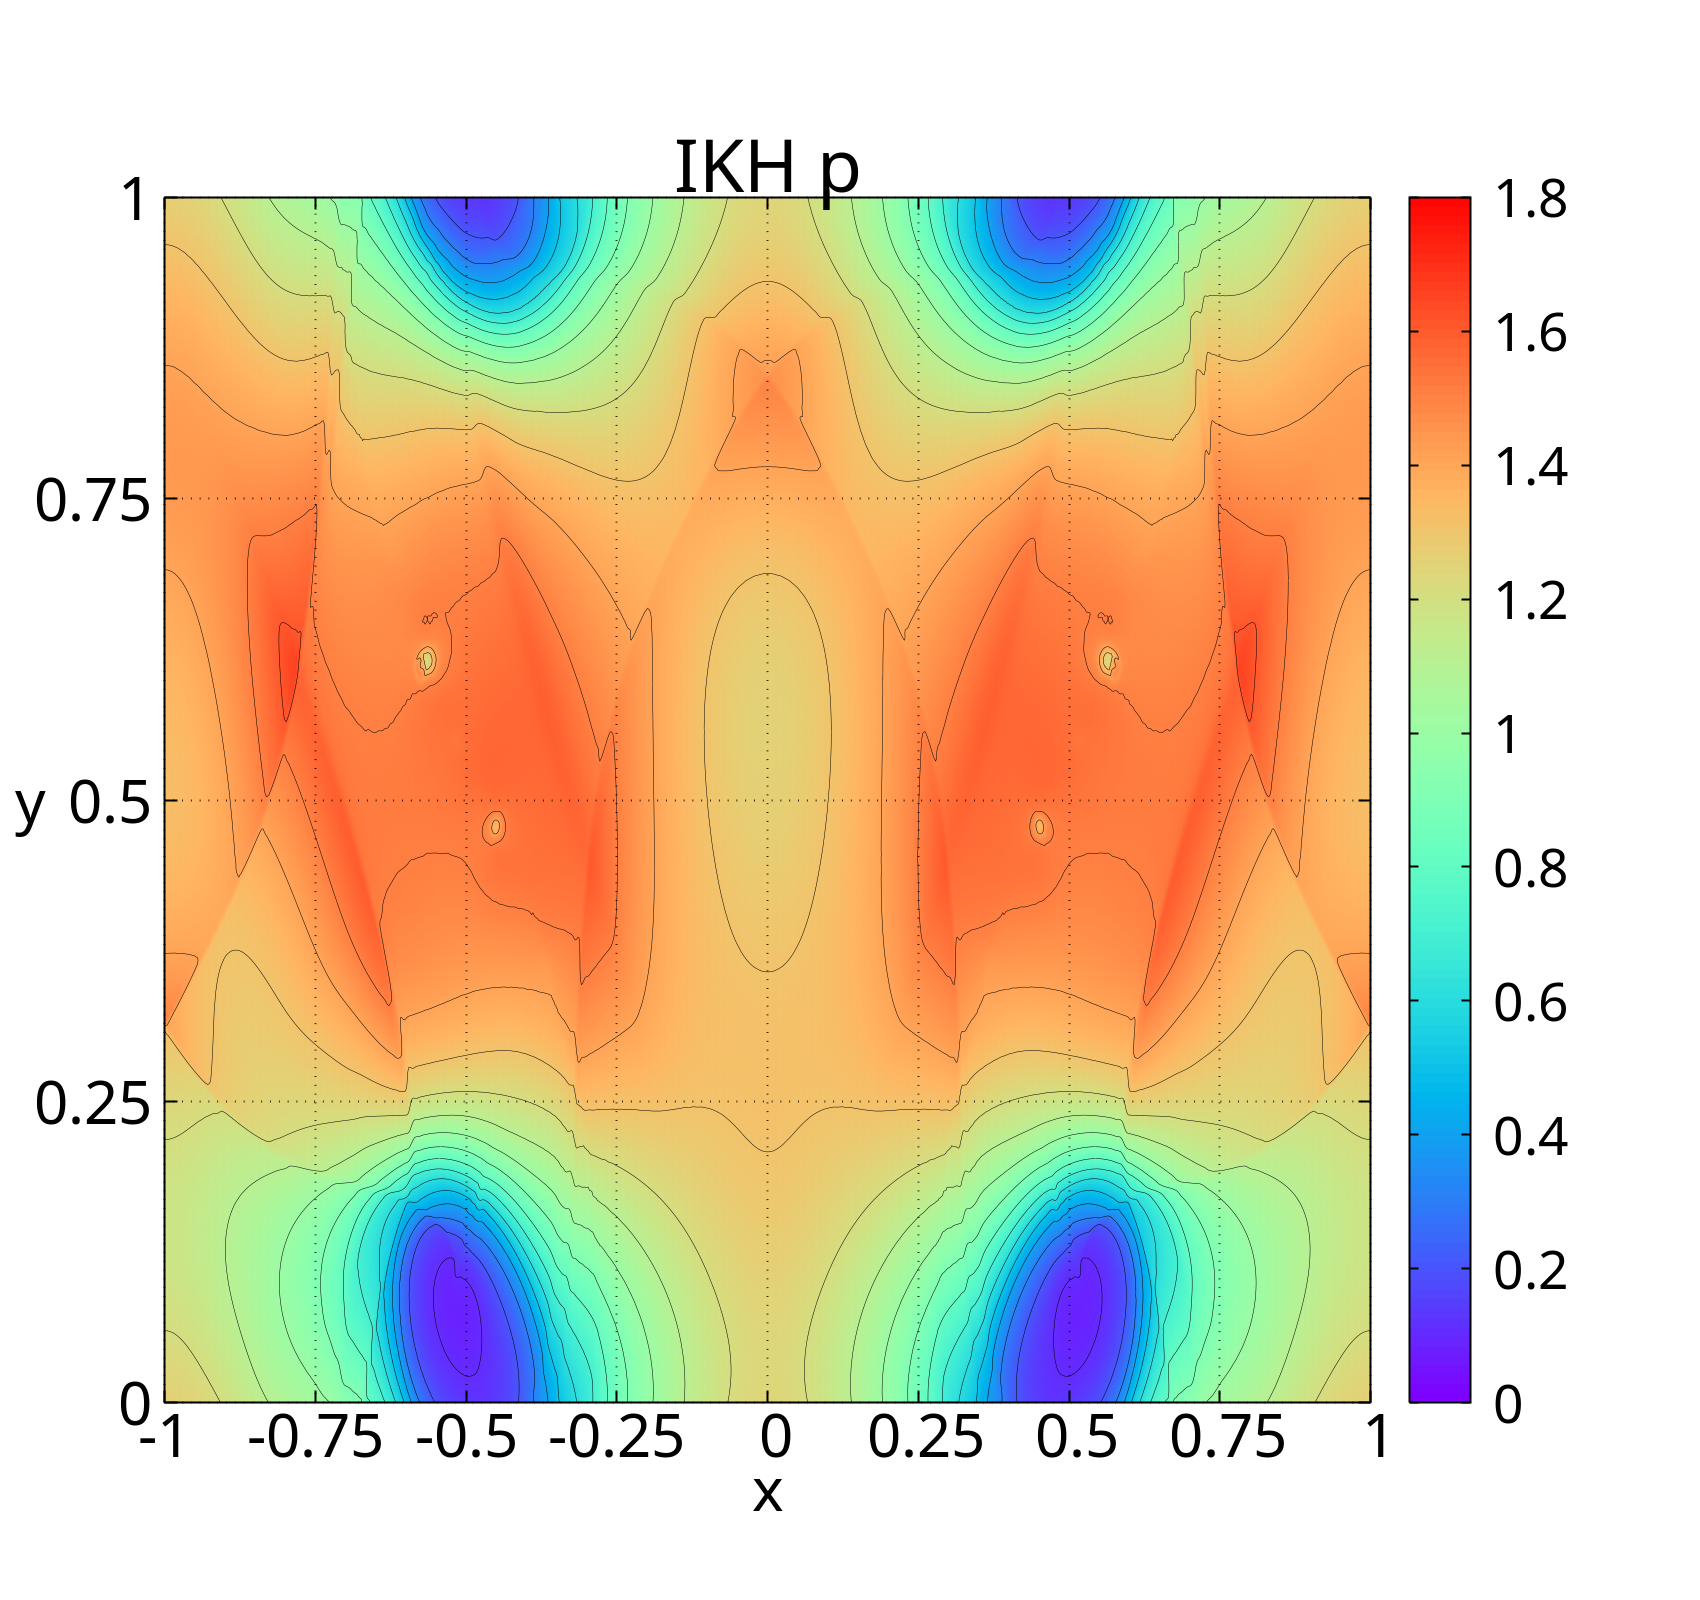
\includegraphics[width=0.24\linewidth]{images/ps1.png}
    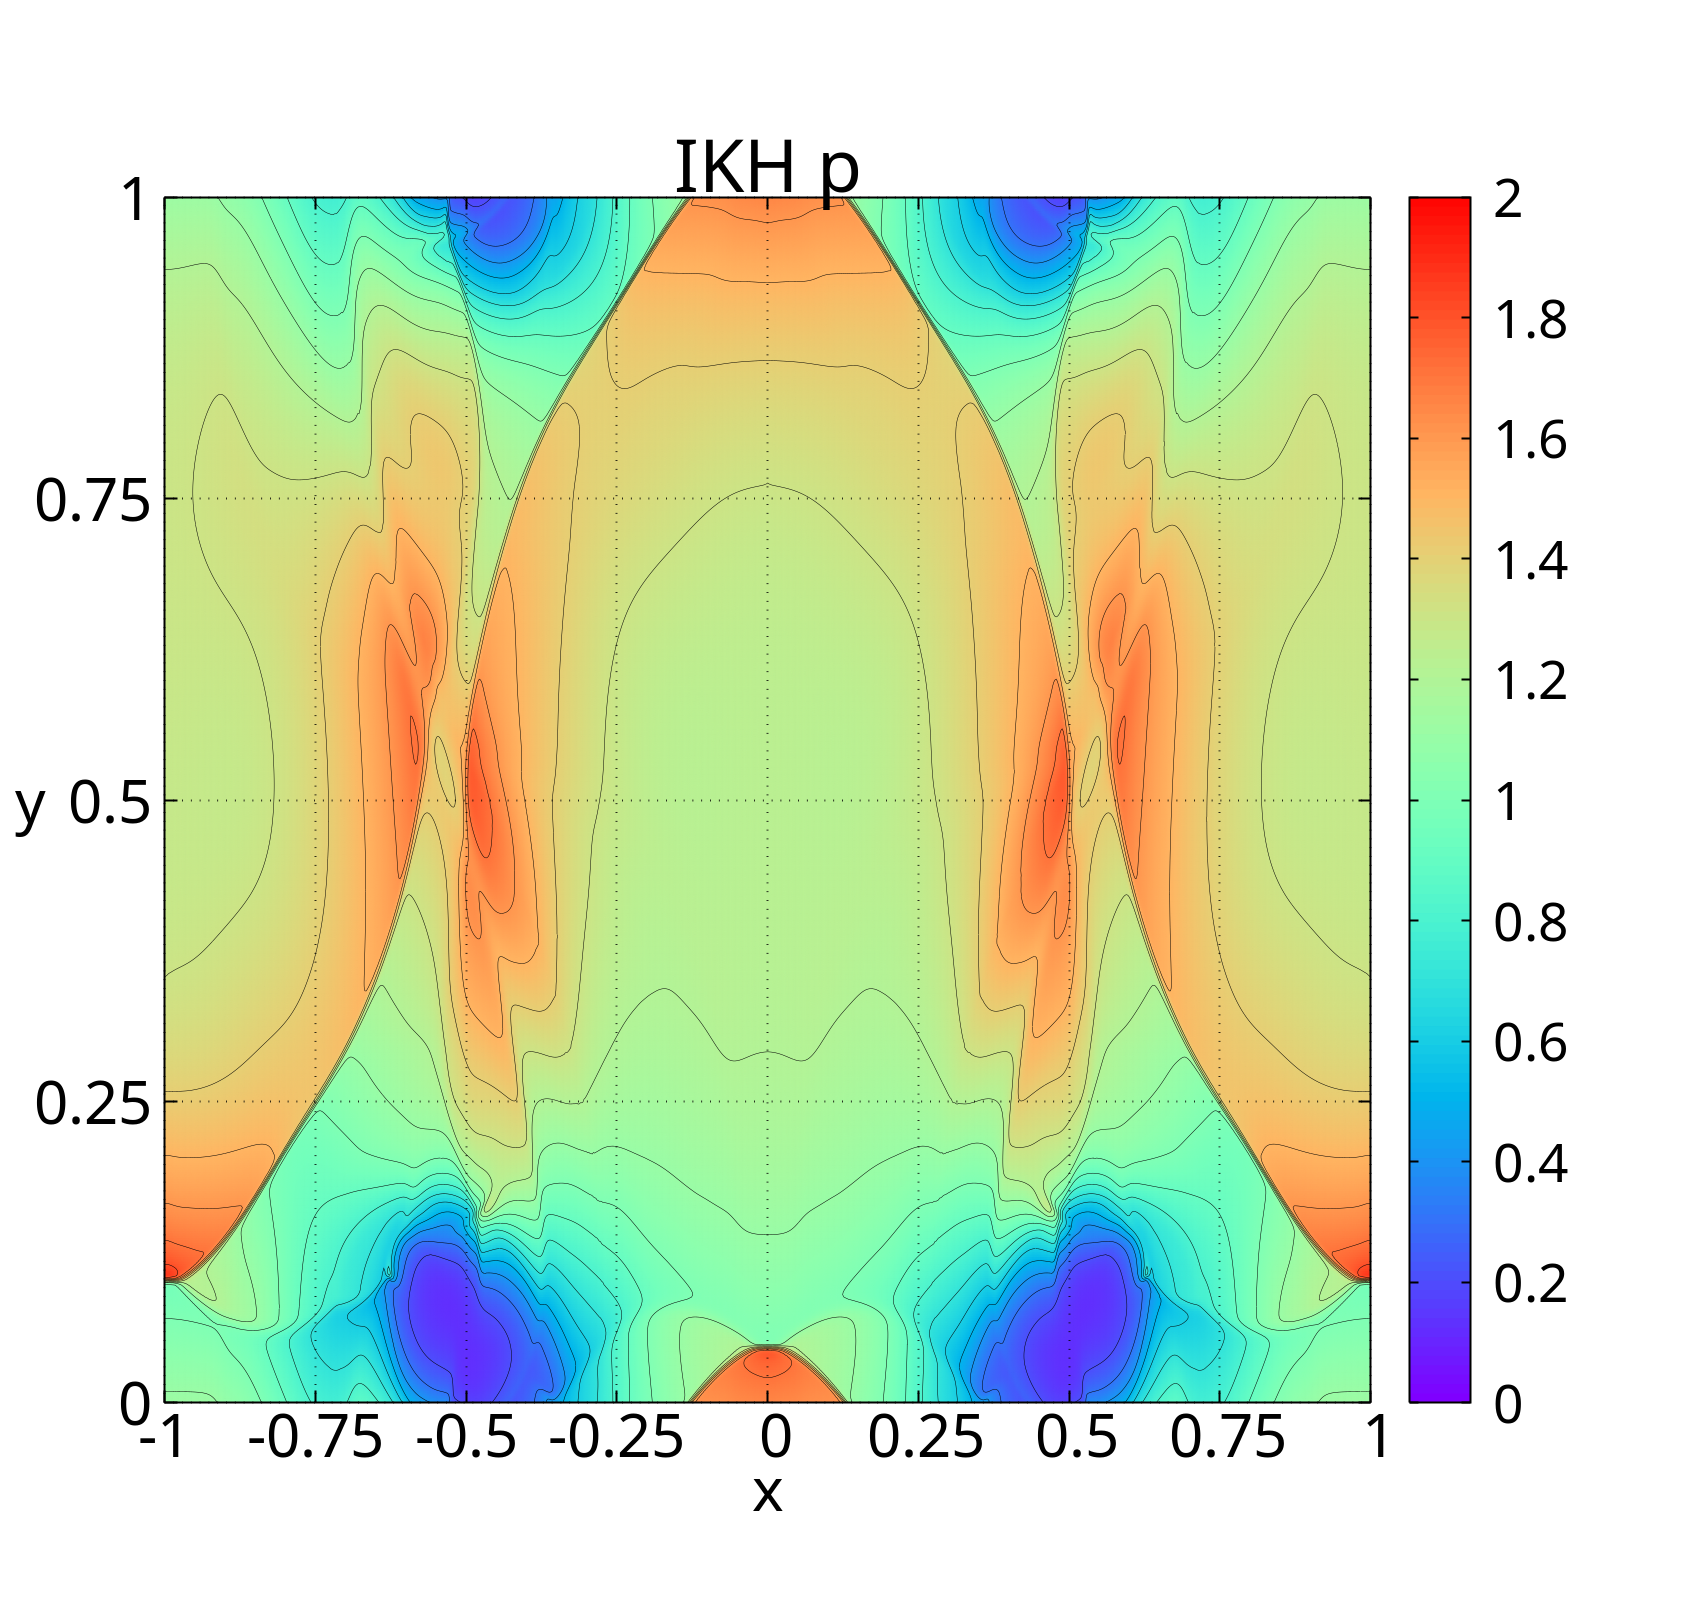
\includegraphics[width=0.24\linewidth]{images/ps3.png}
    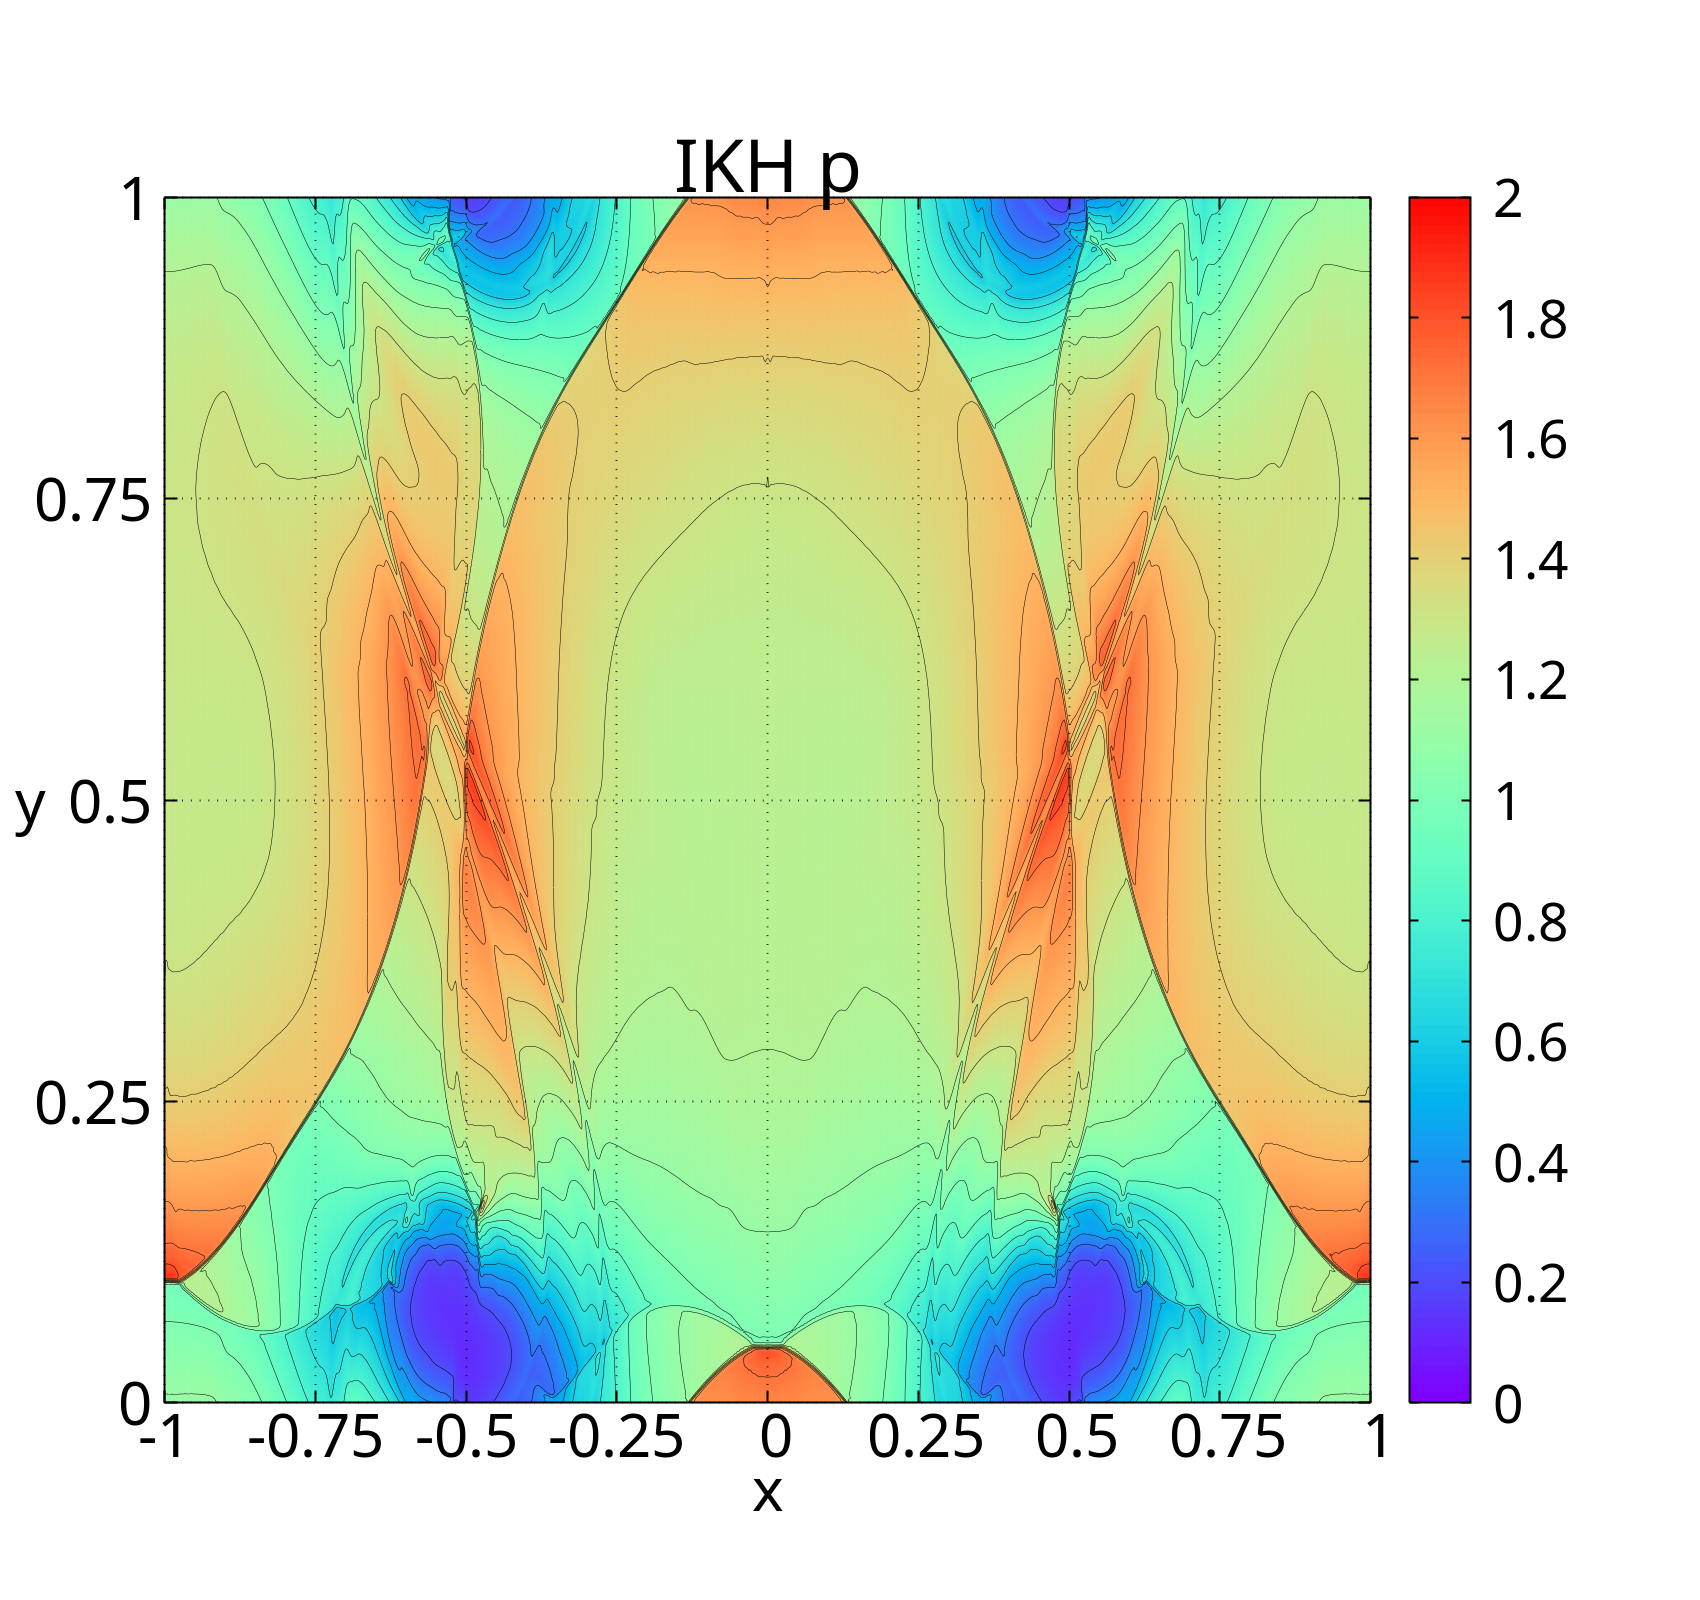
\includegraphics[width=0.24\linewidth]{images/ps6.png}
    \vspace*{-0.5cm}
    \caption{Presión para diferentes valores de conductividad}
    \vspace*{-0.8cm}
    \end{figure}
    
    \begin{figure}[H]
    \centering
    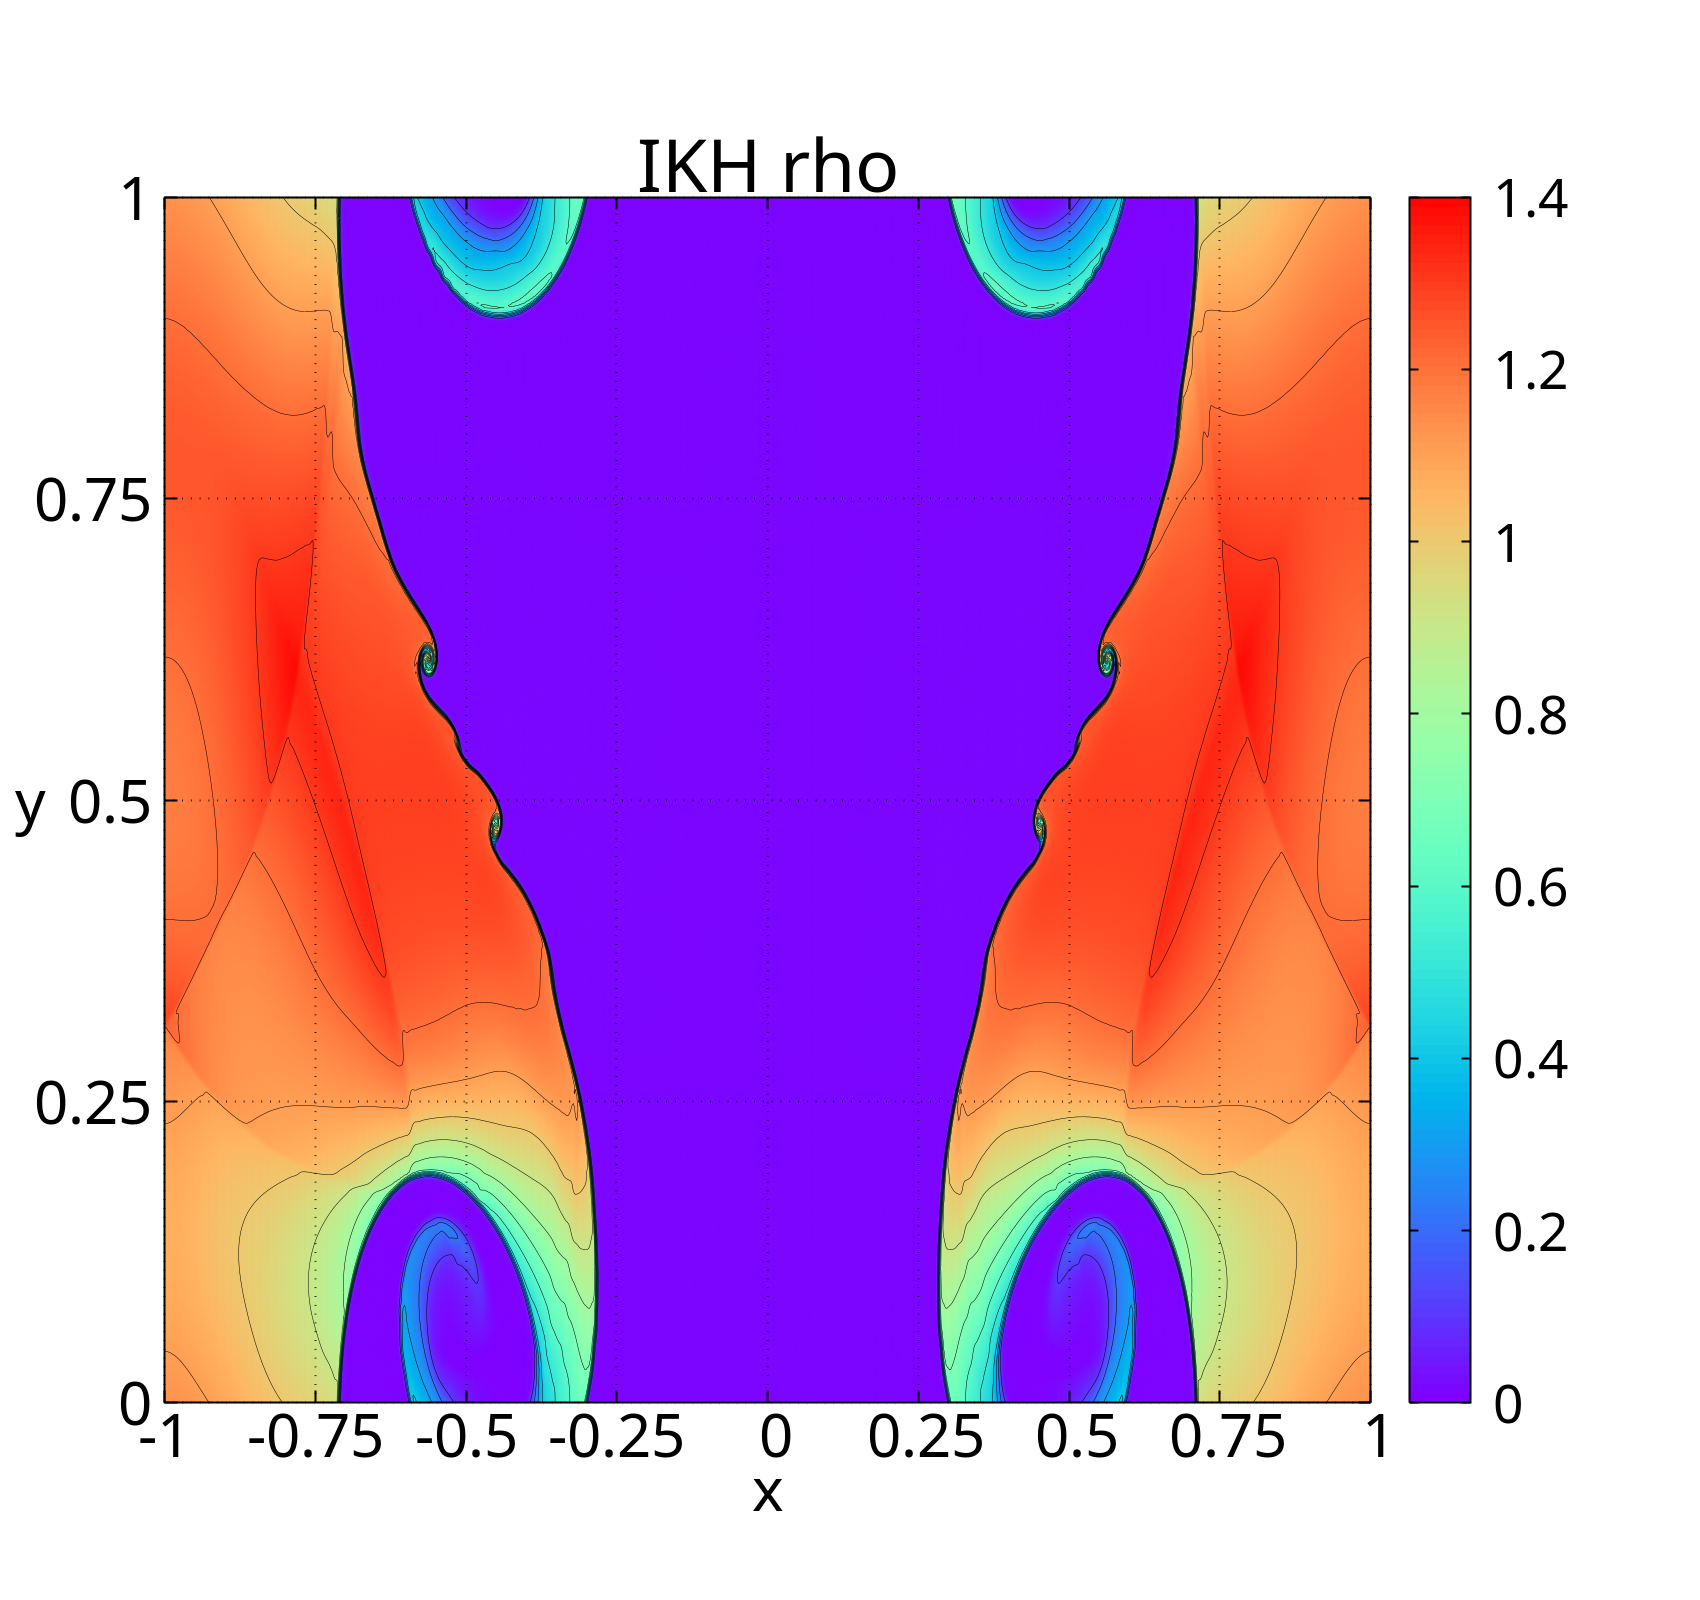
\includegraphics[width=0.24\linewidth]{images/rhos1.png}
    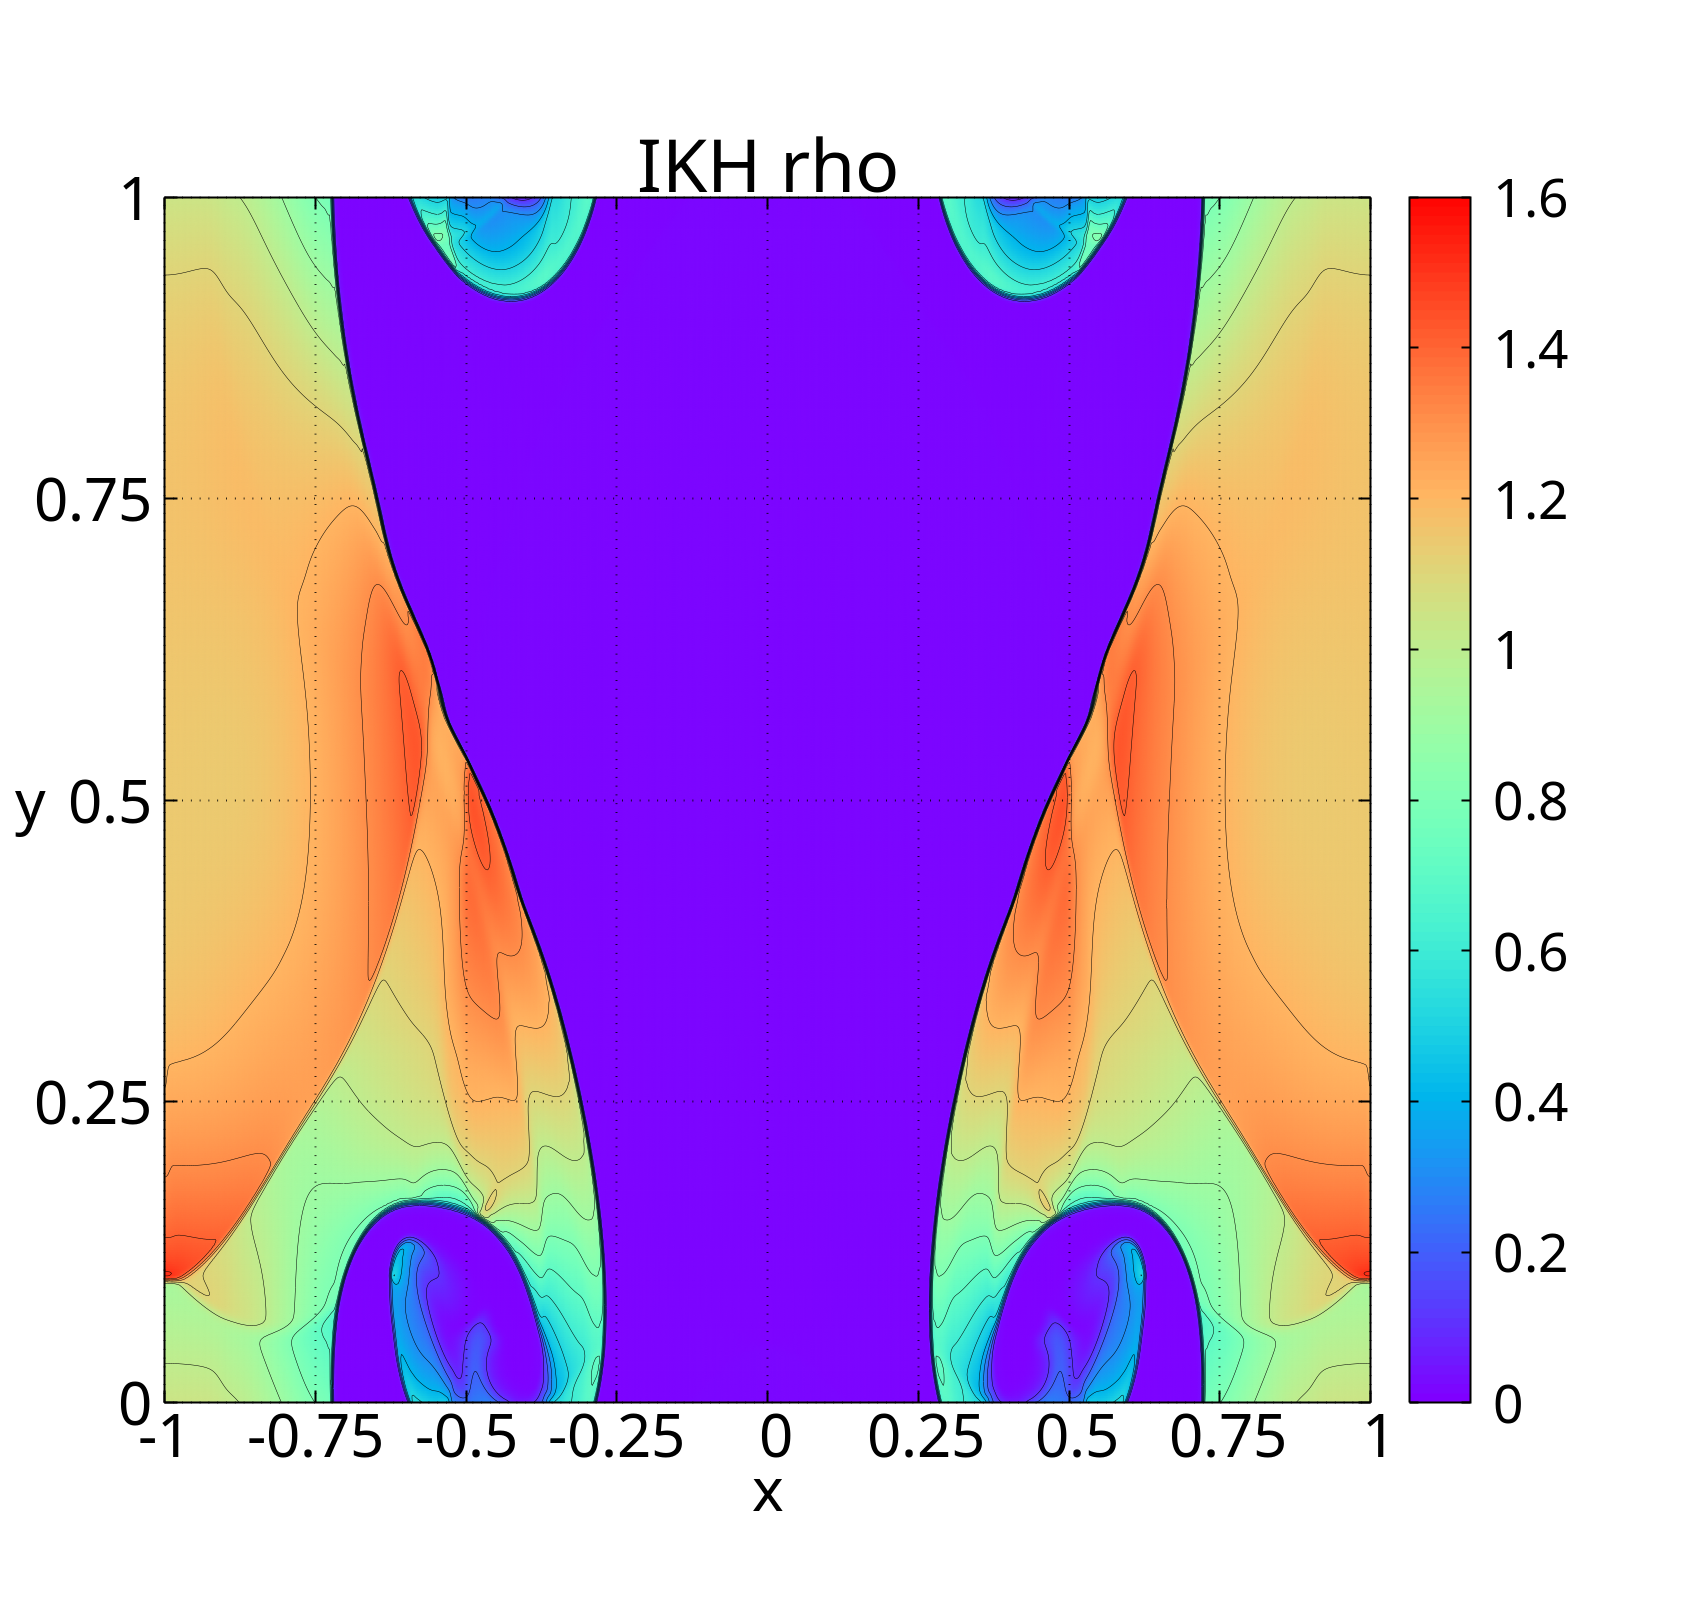
\includegraphics[width=0.24\linewidth]{images/rhos3.png}
    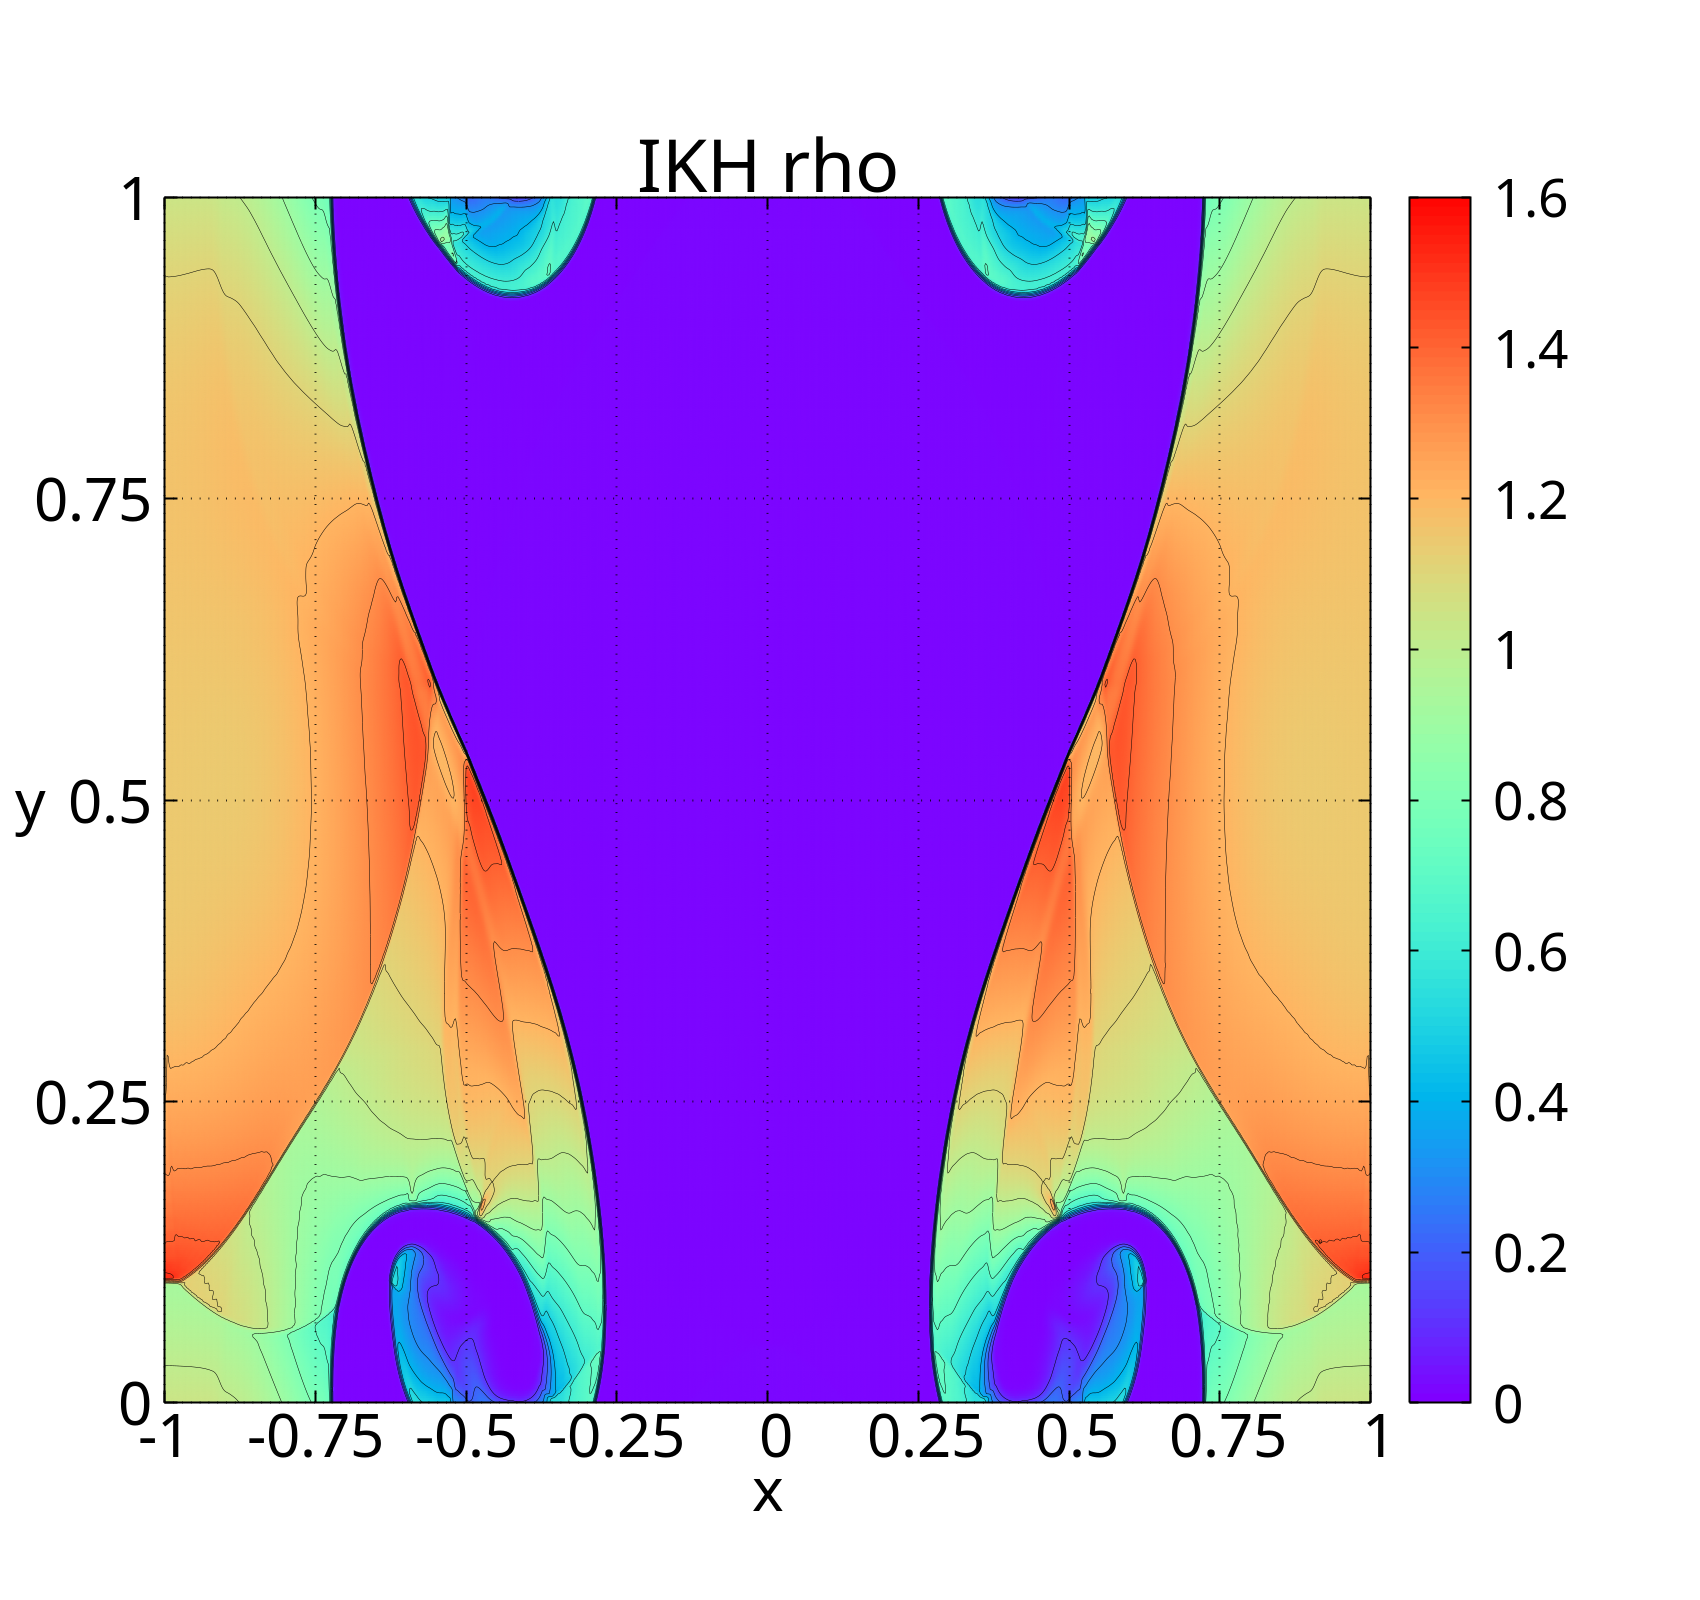
\includegraphics[width=0.24\linewidth]{images/rhos6.png}
    \vspace*{-0.5cm}
    \caption{Densidad para diferentes valores de conductividad}
    \vspace*{-0.8cm}
    \end{figure}
    
    \begin{figure}[H]
    \centering
    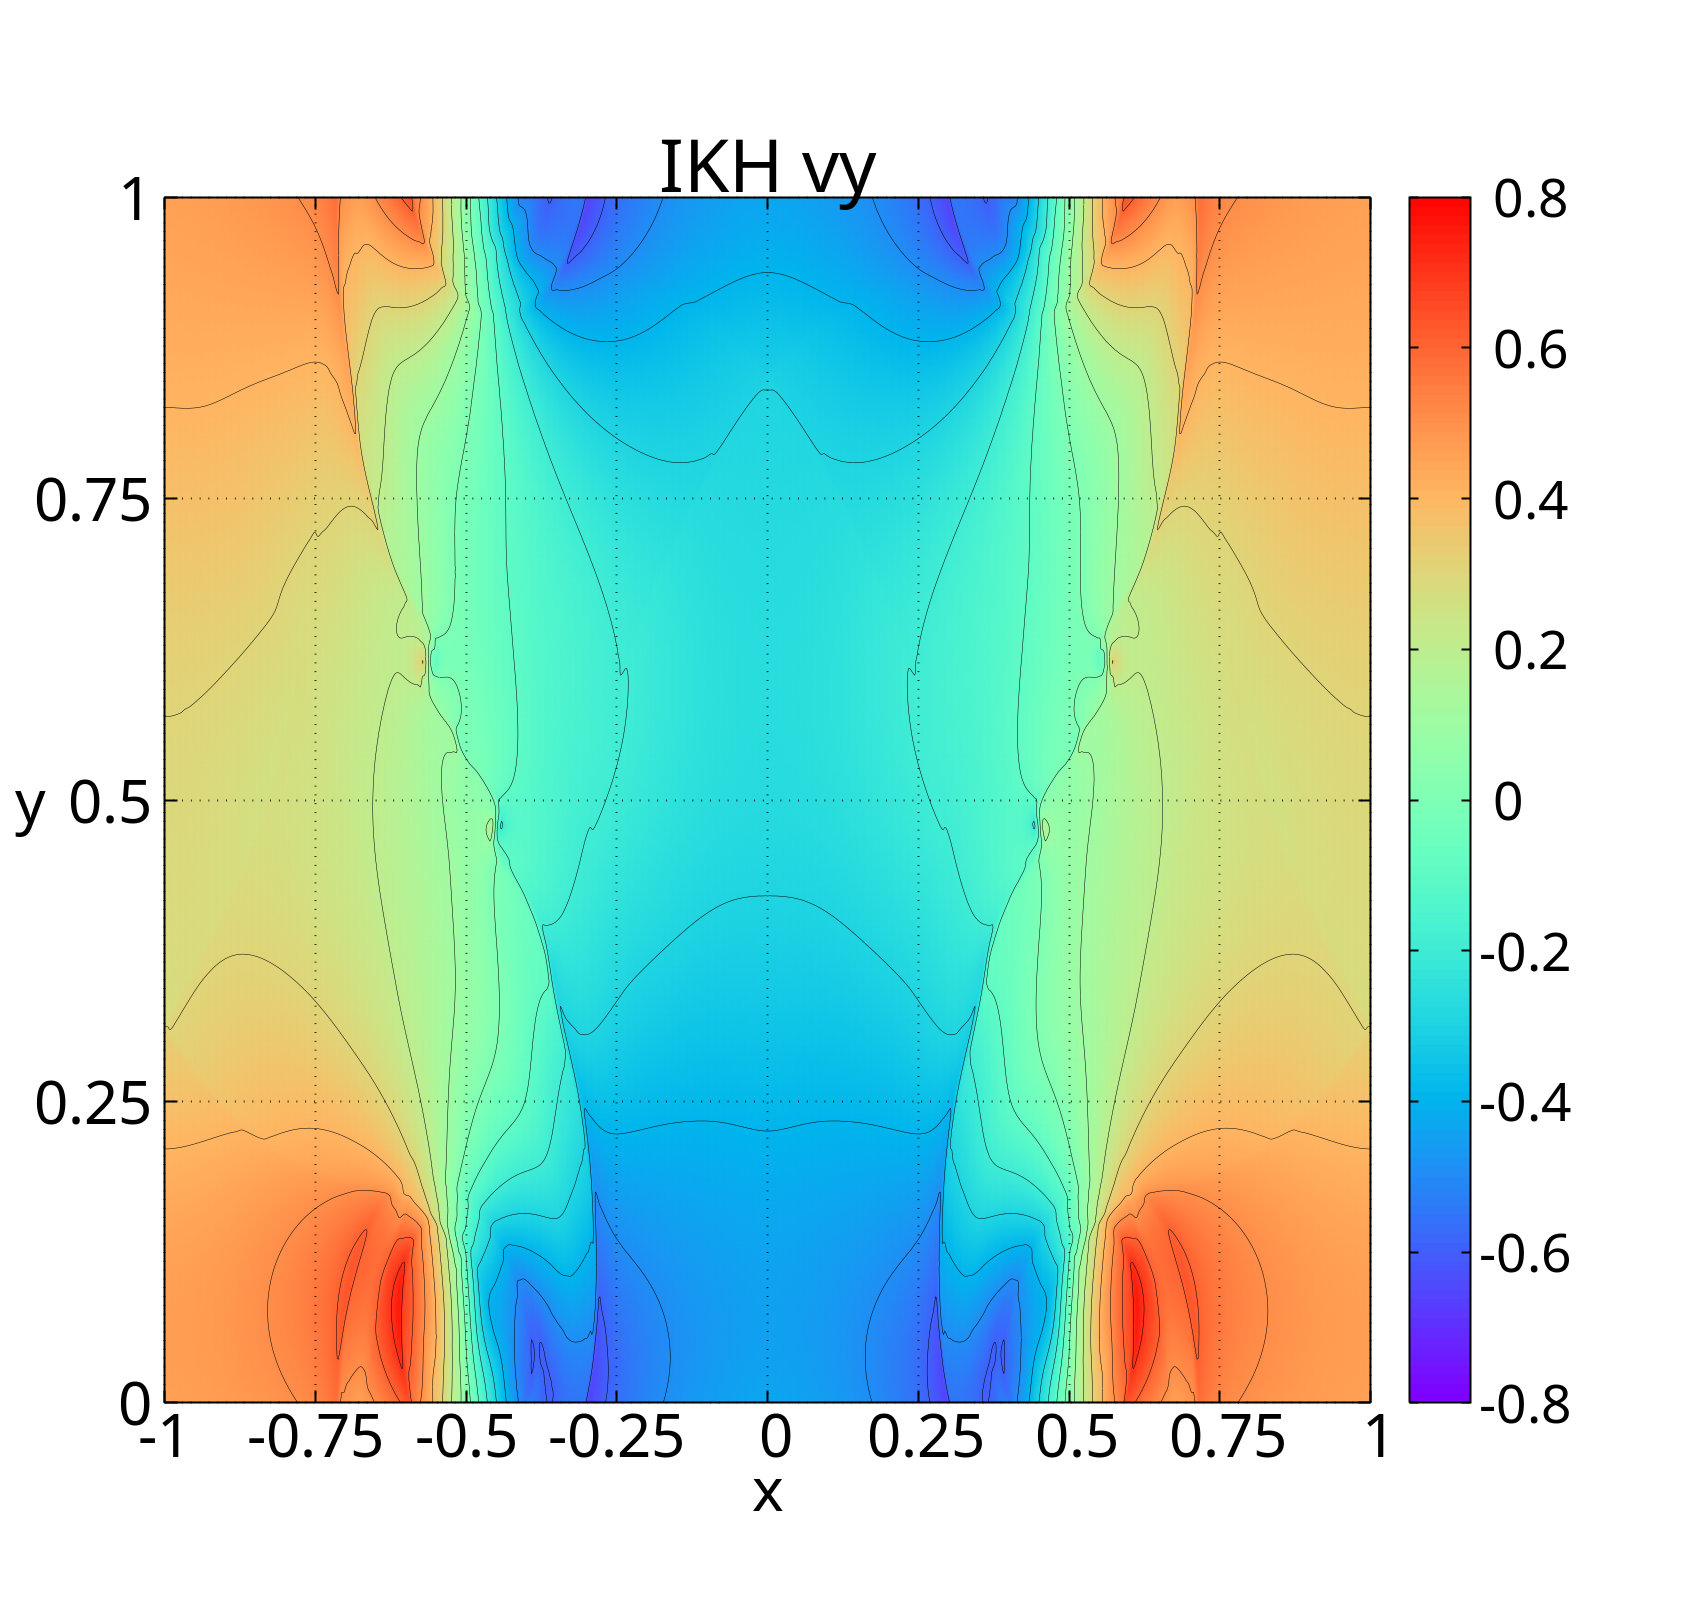
\includegraphics[width=0.24\linewidth]{images/vys1.png}
    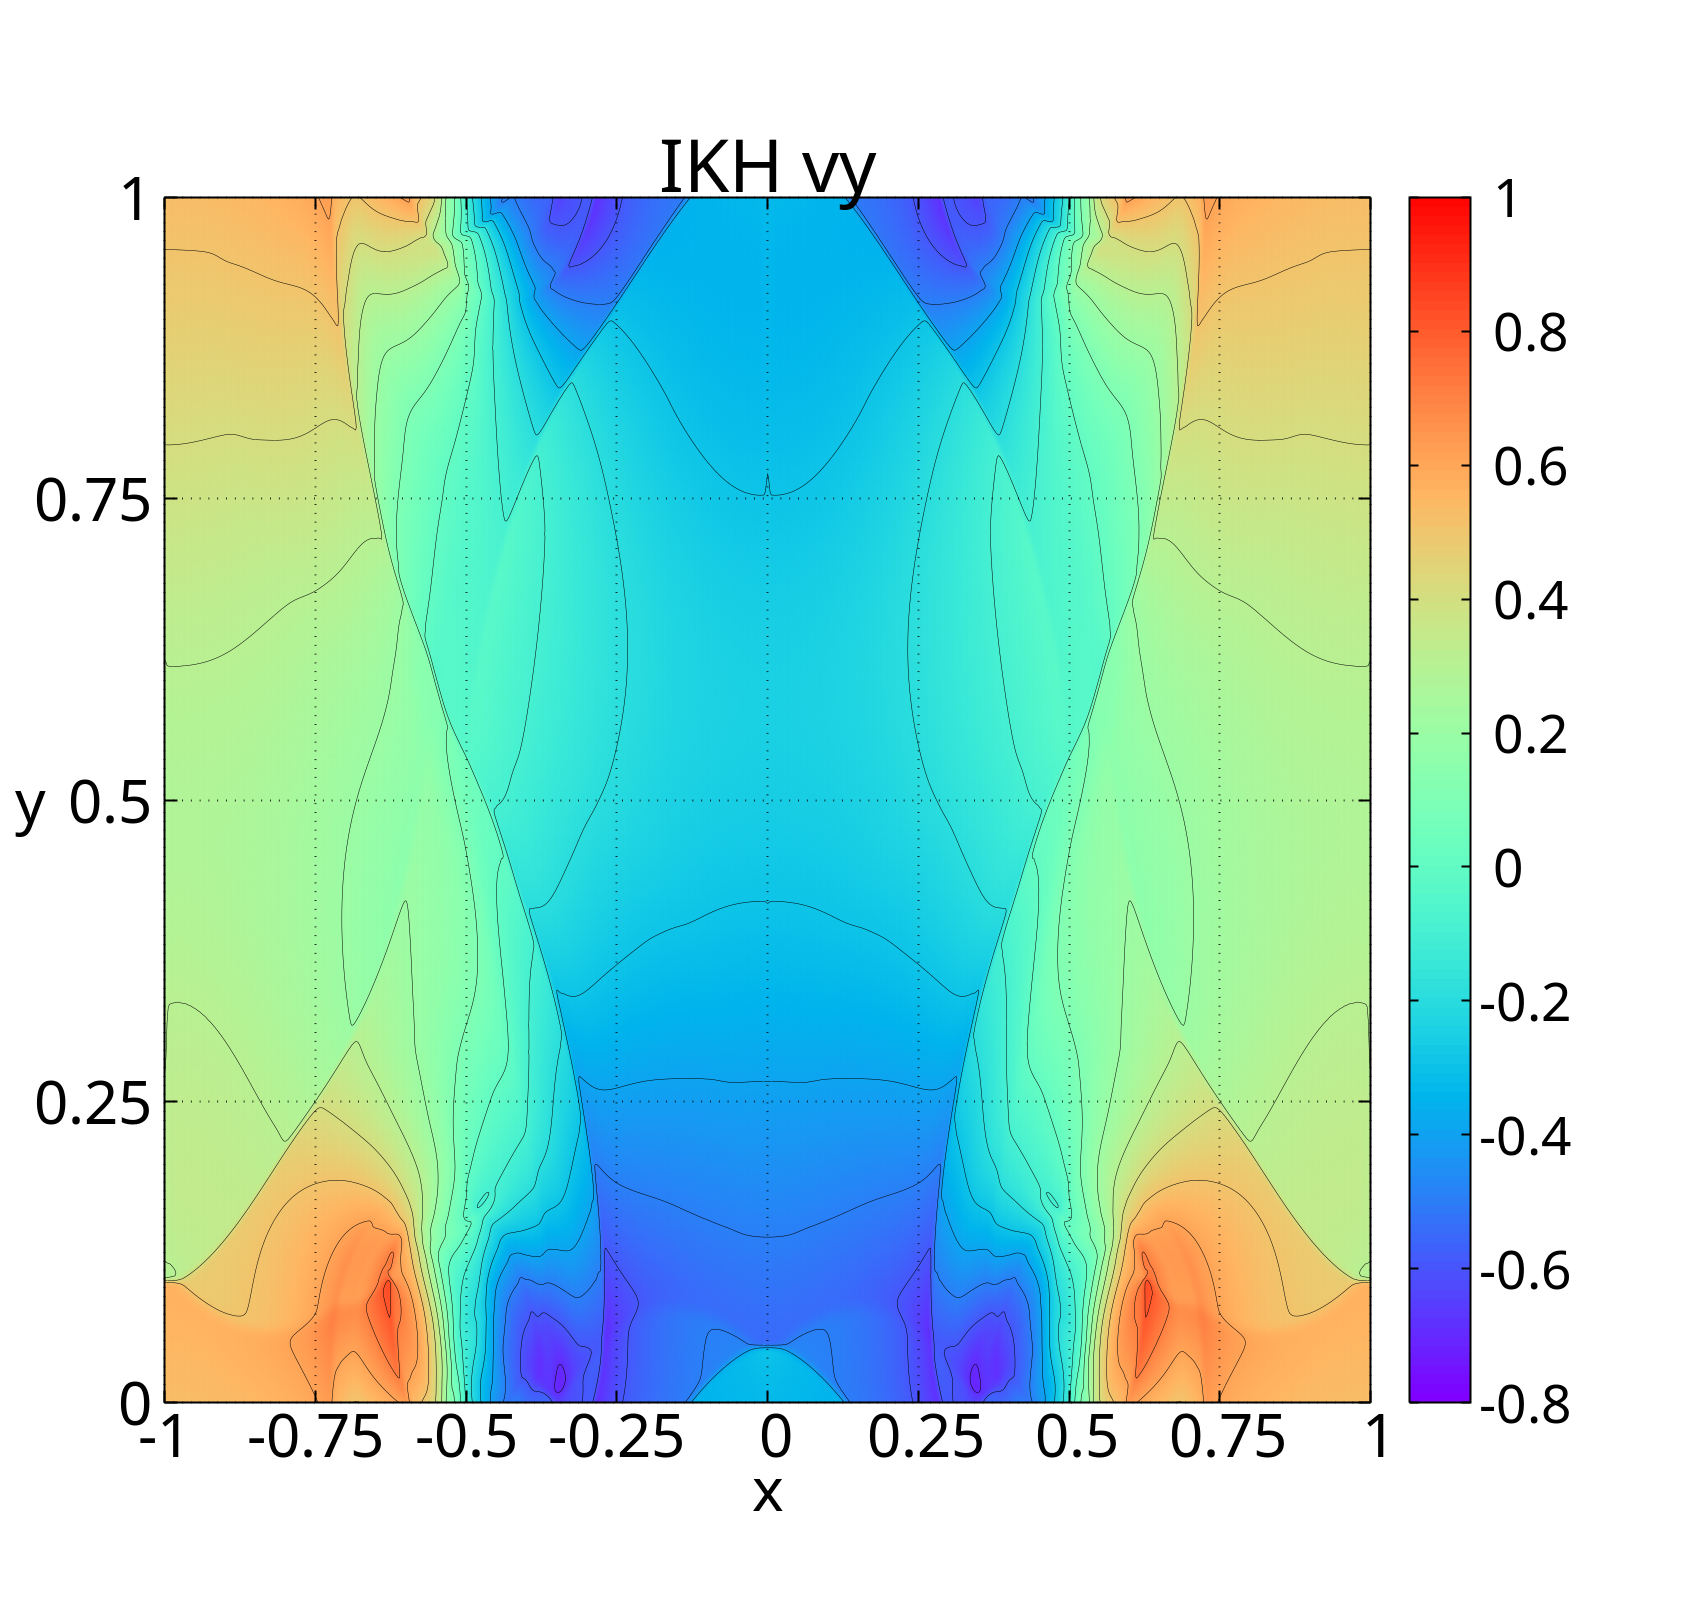
\includegraphics[width=0.24\linewidth]{images/vys3.png}
    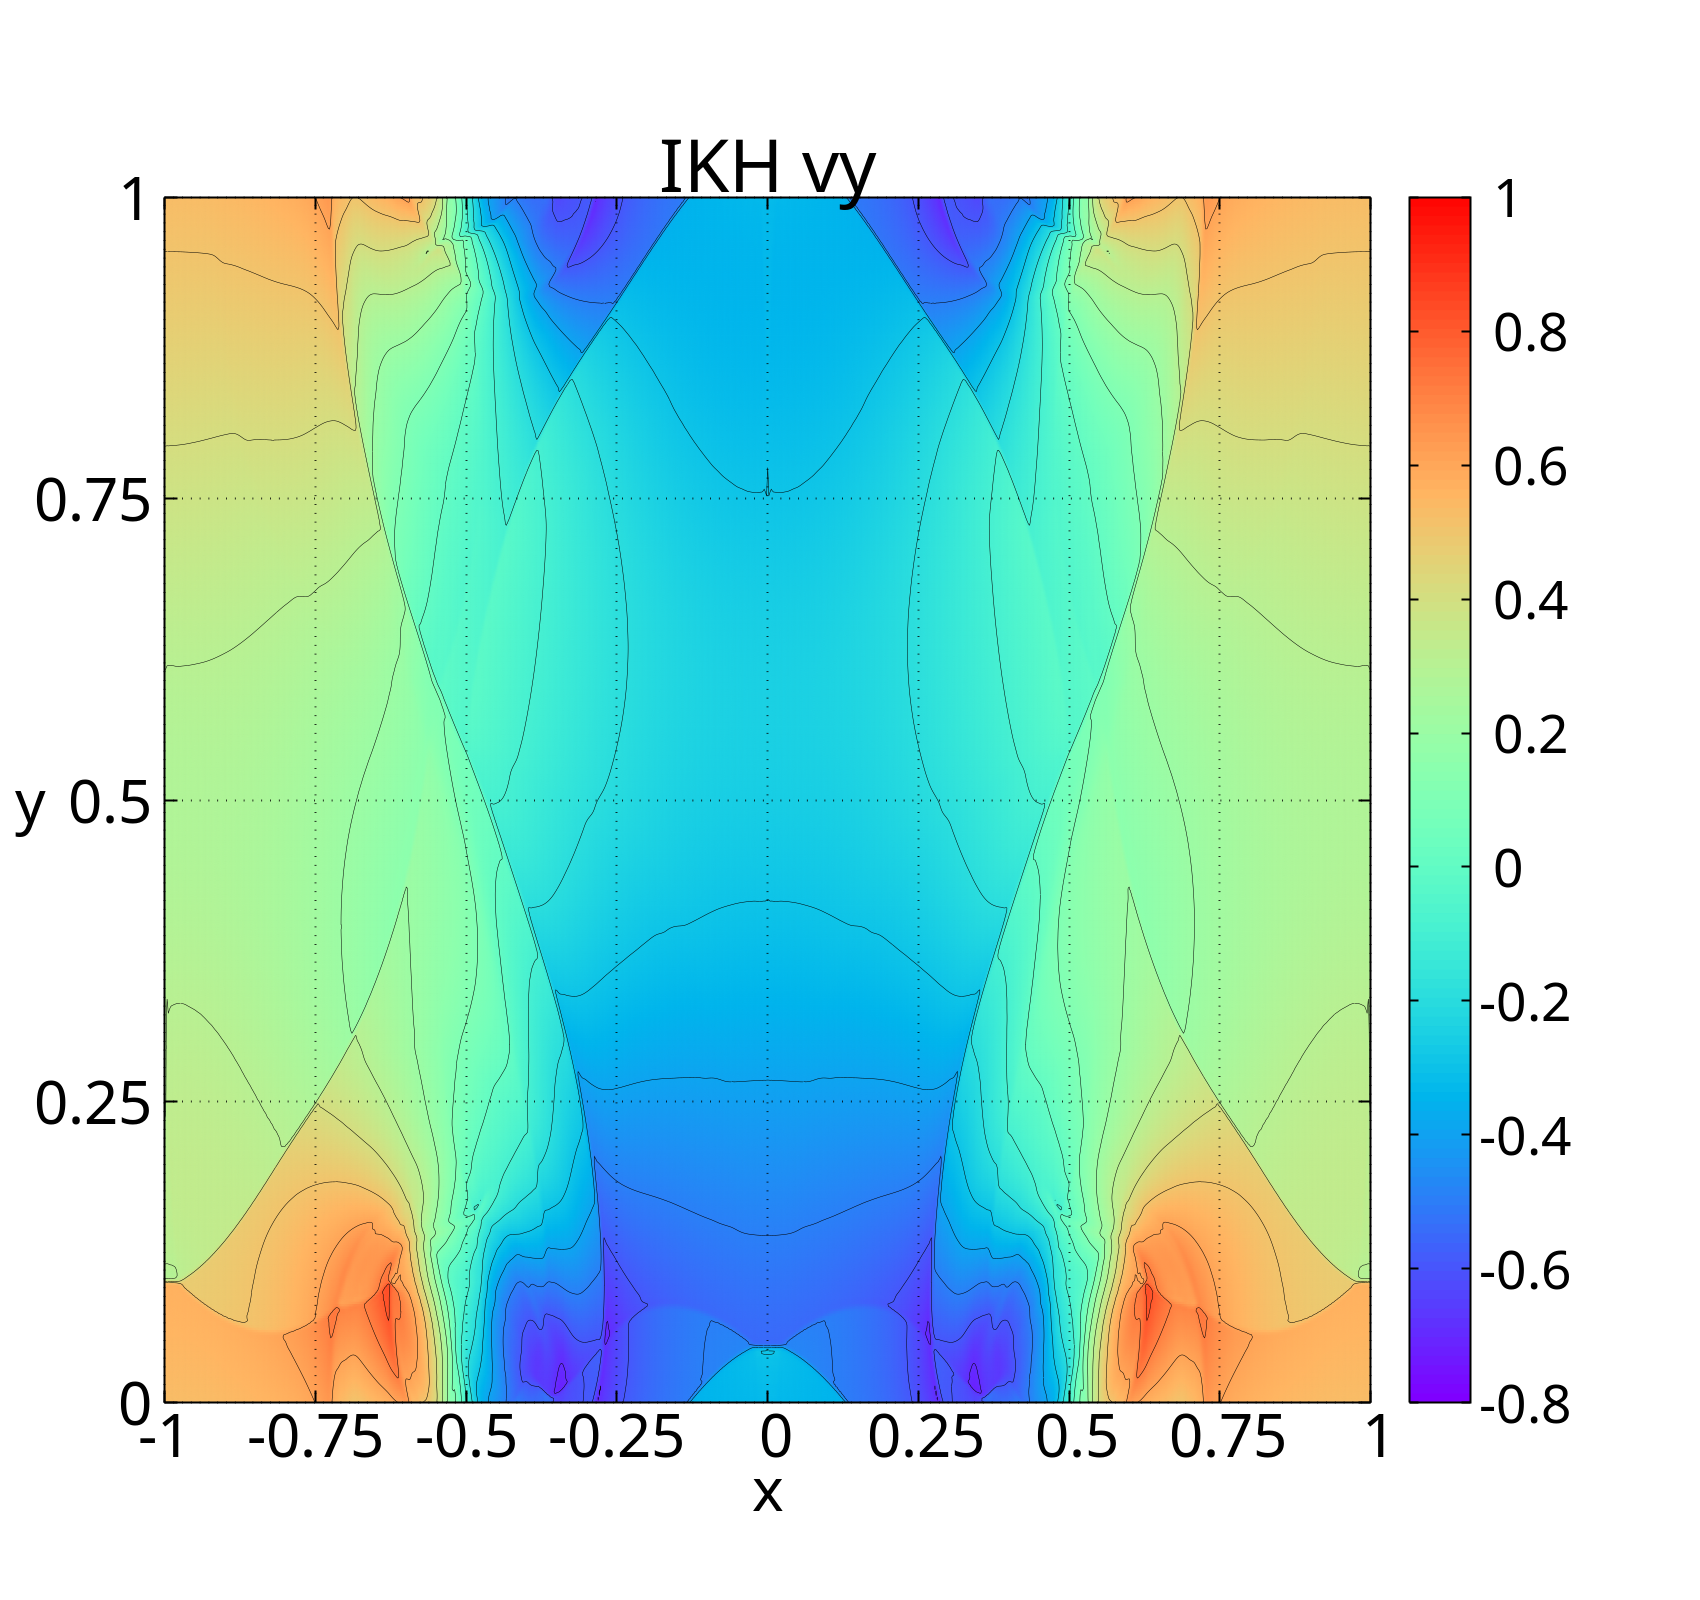
\includegraphics[width=0.24\linewidth]{images/vys6.png}
    \vspace*{-0.5cm}
    \caption{Velocidad en y para diferentes valores de conductividad}
    \vspace*{-0.8cm}
    \end{figure}
    
    \begin{figure}[H]
    \centering
    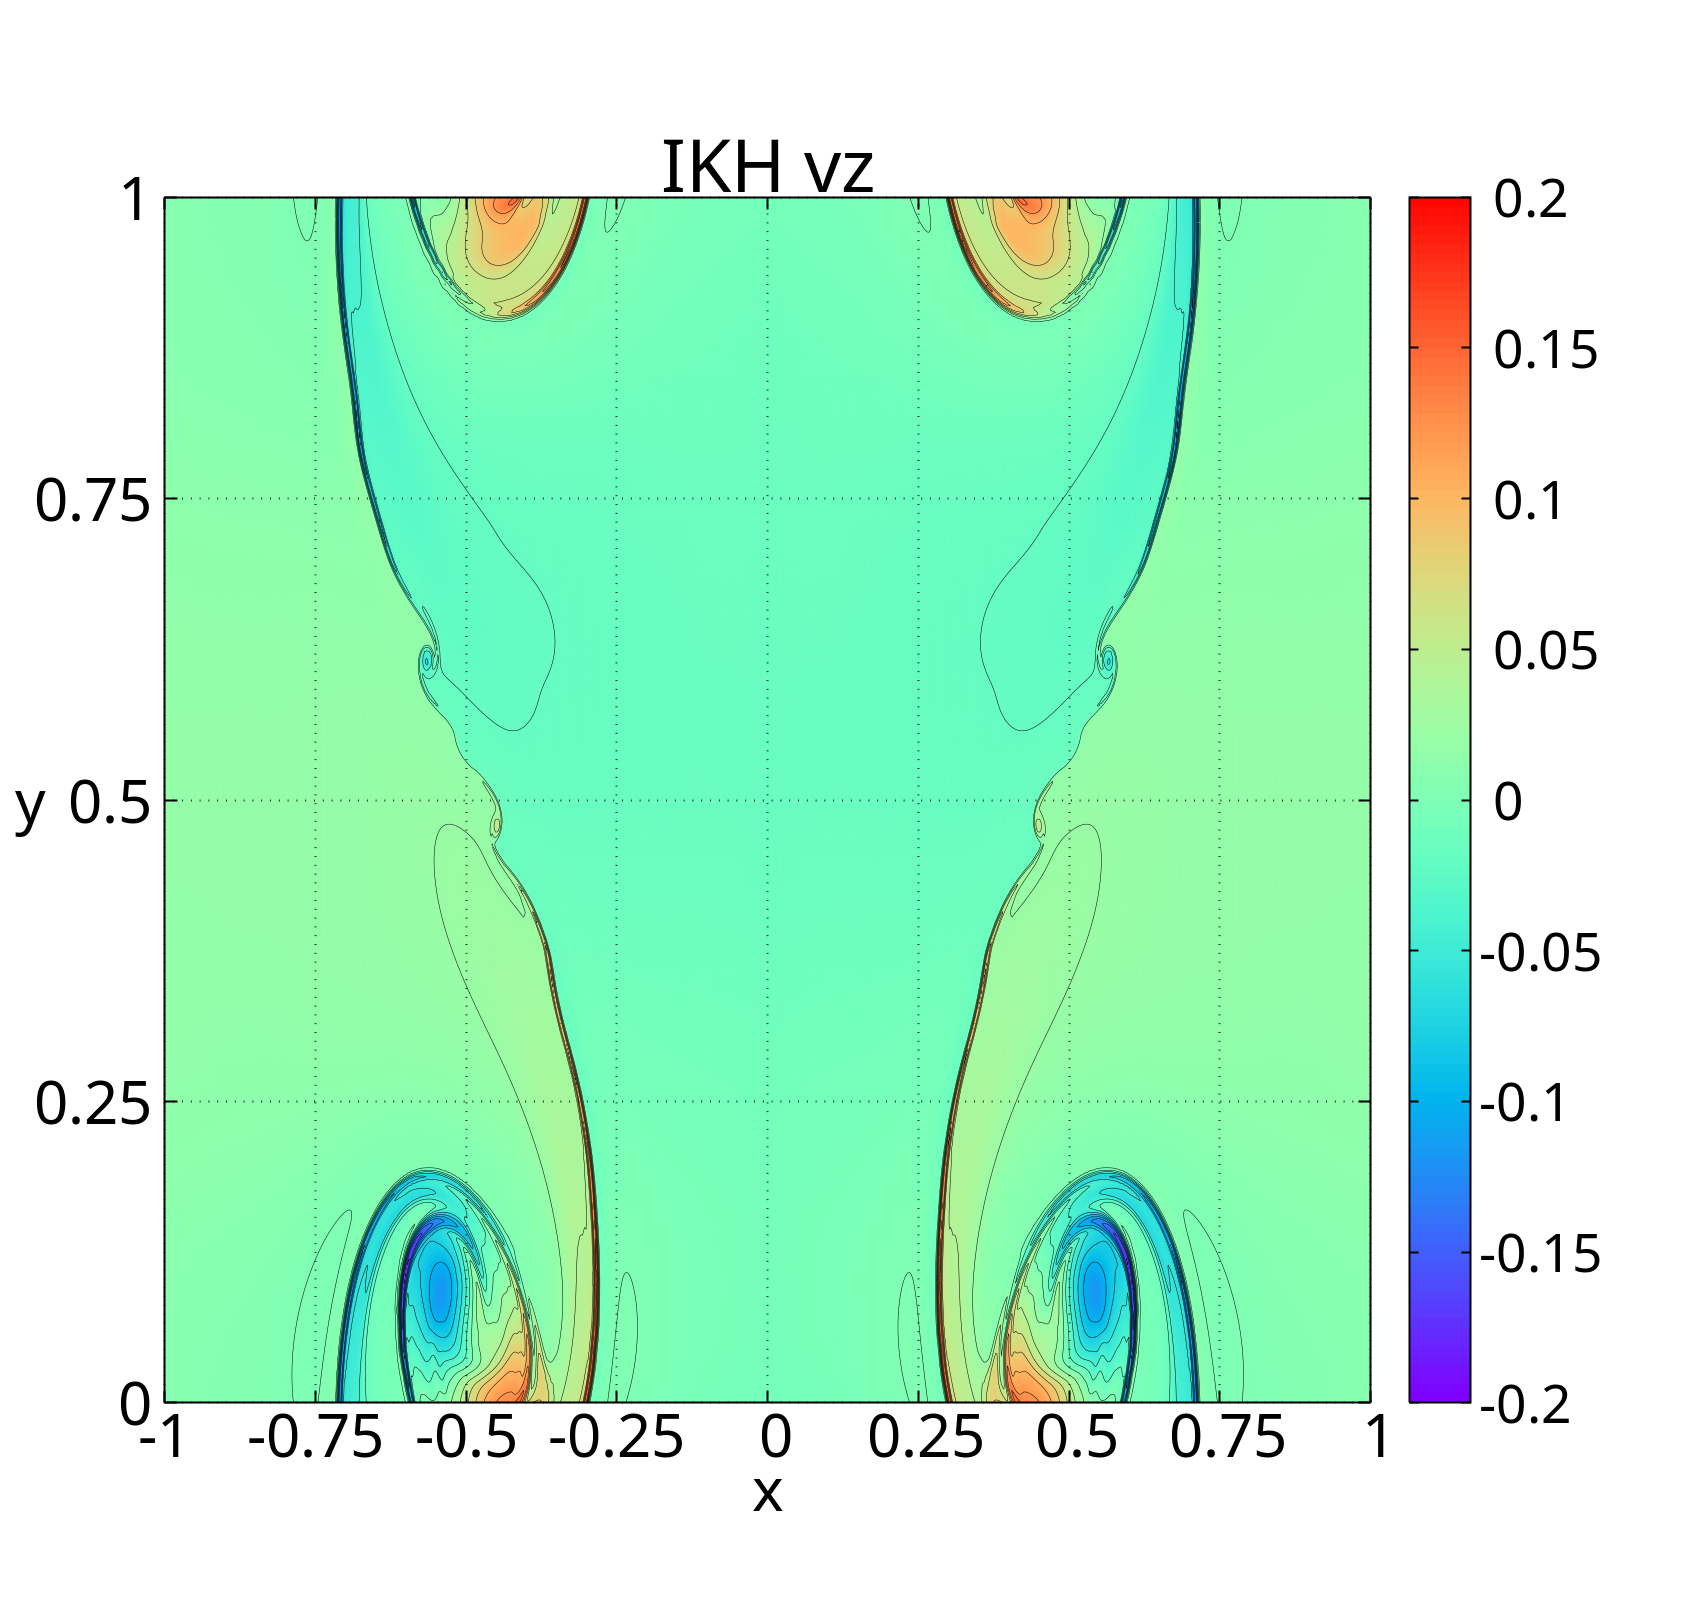
\includegraphics[width=0.24\linewidth]{images/vzs1.png}
    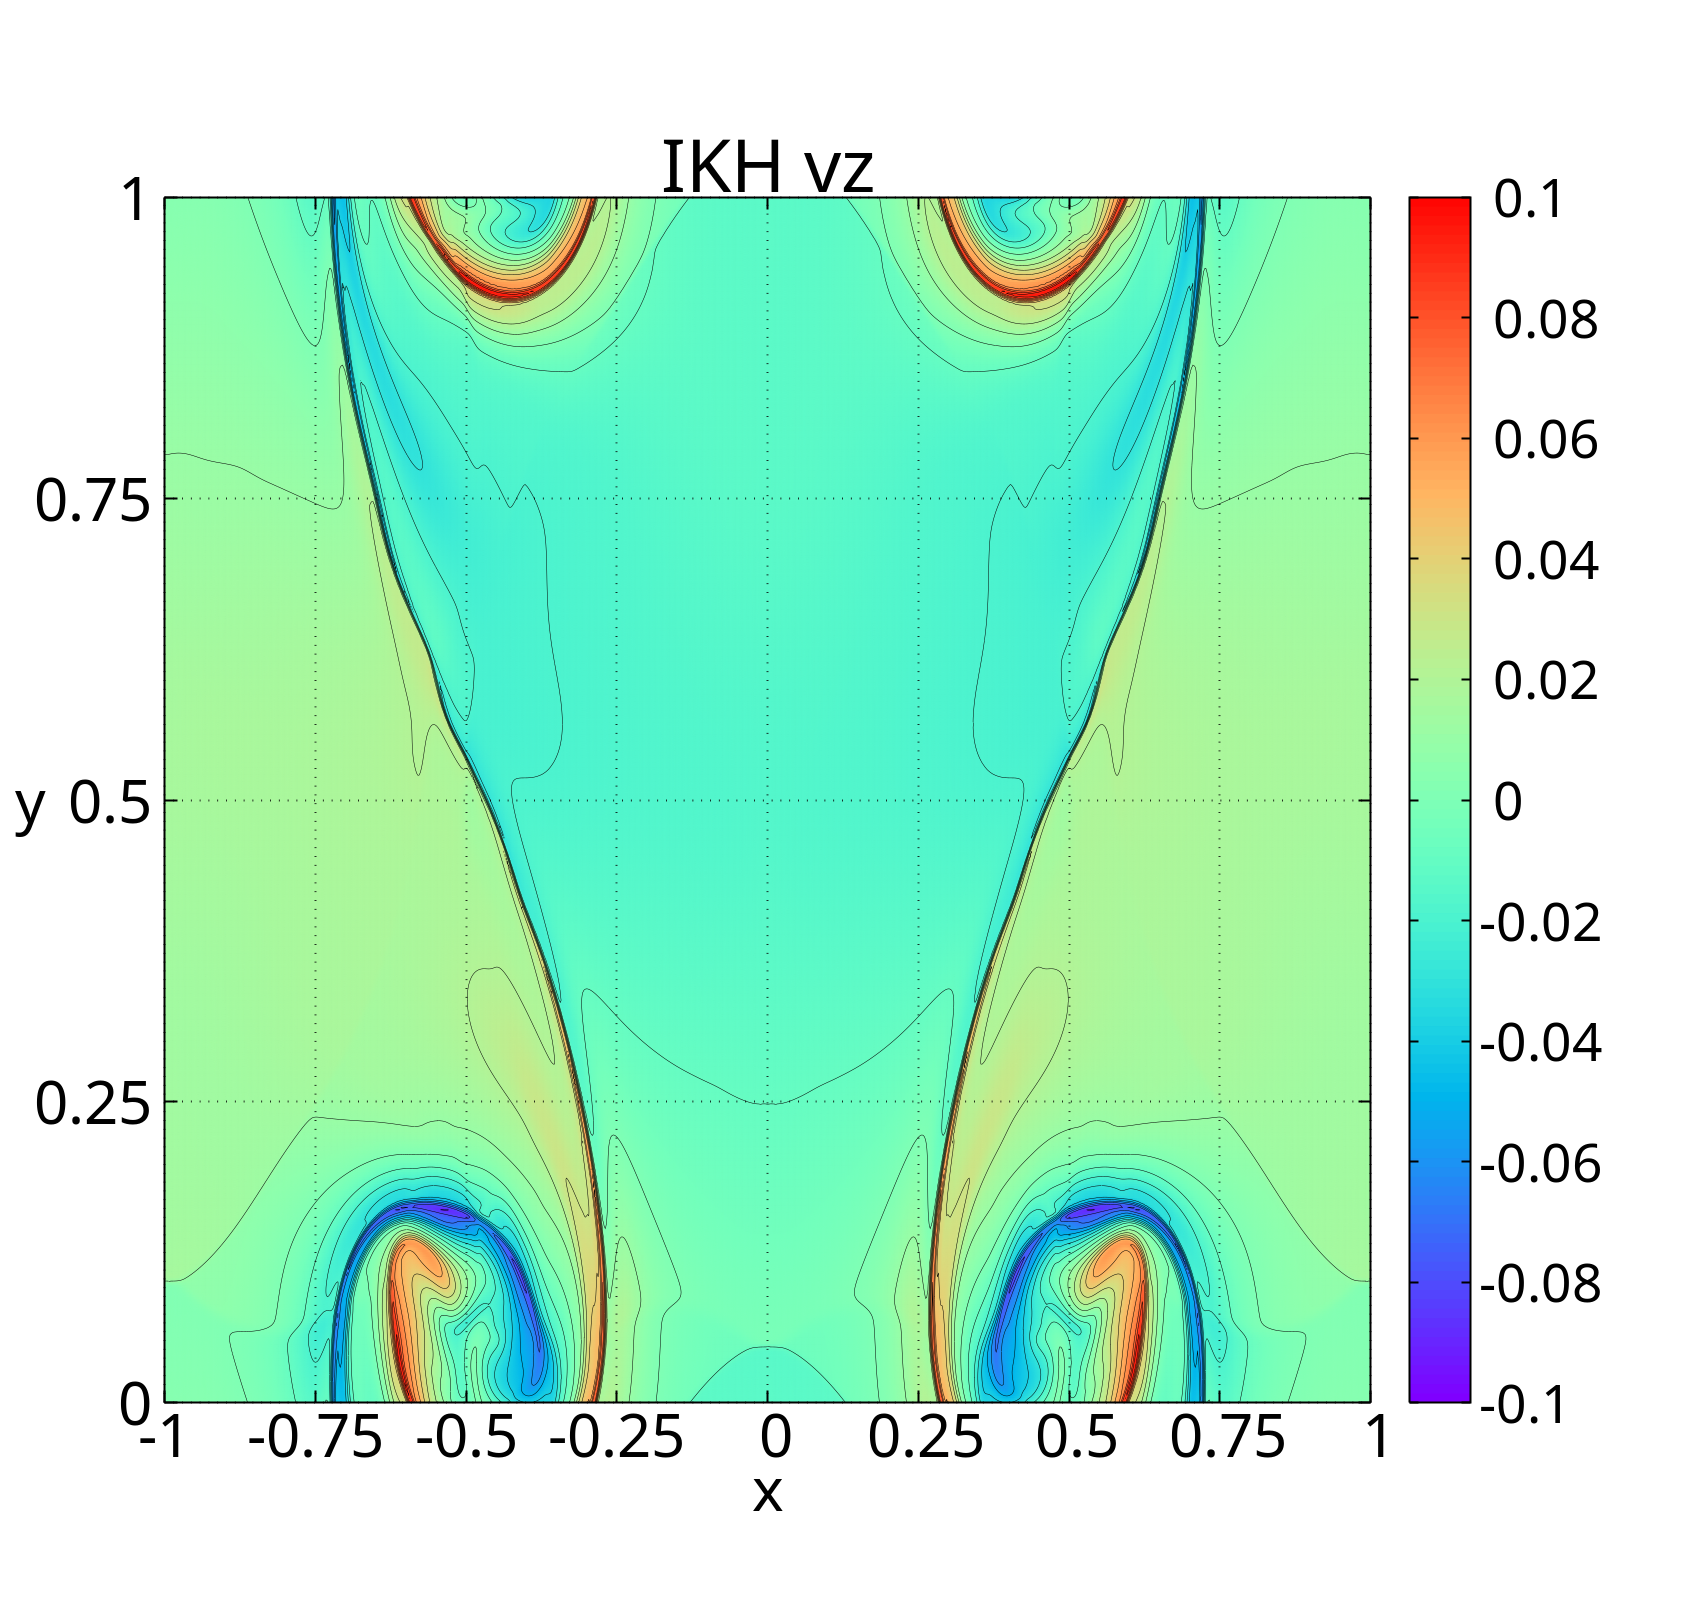
\includegraphics[width=0.24\linewidth]{images/vzs3.png}
    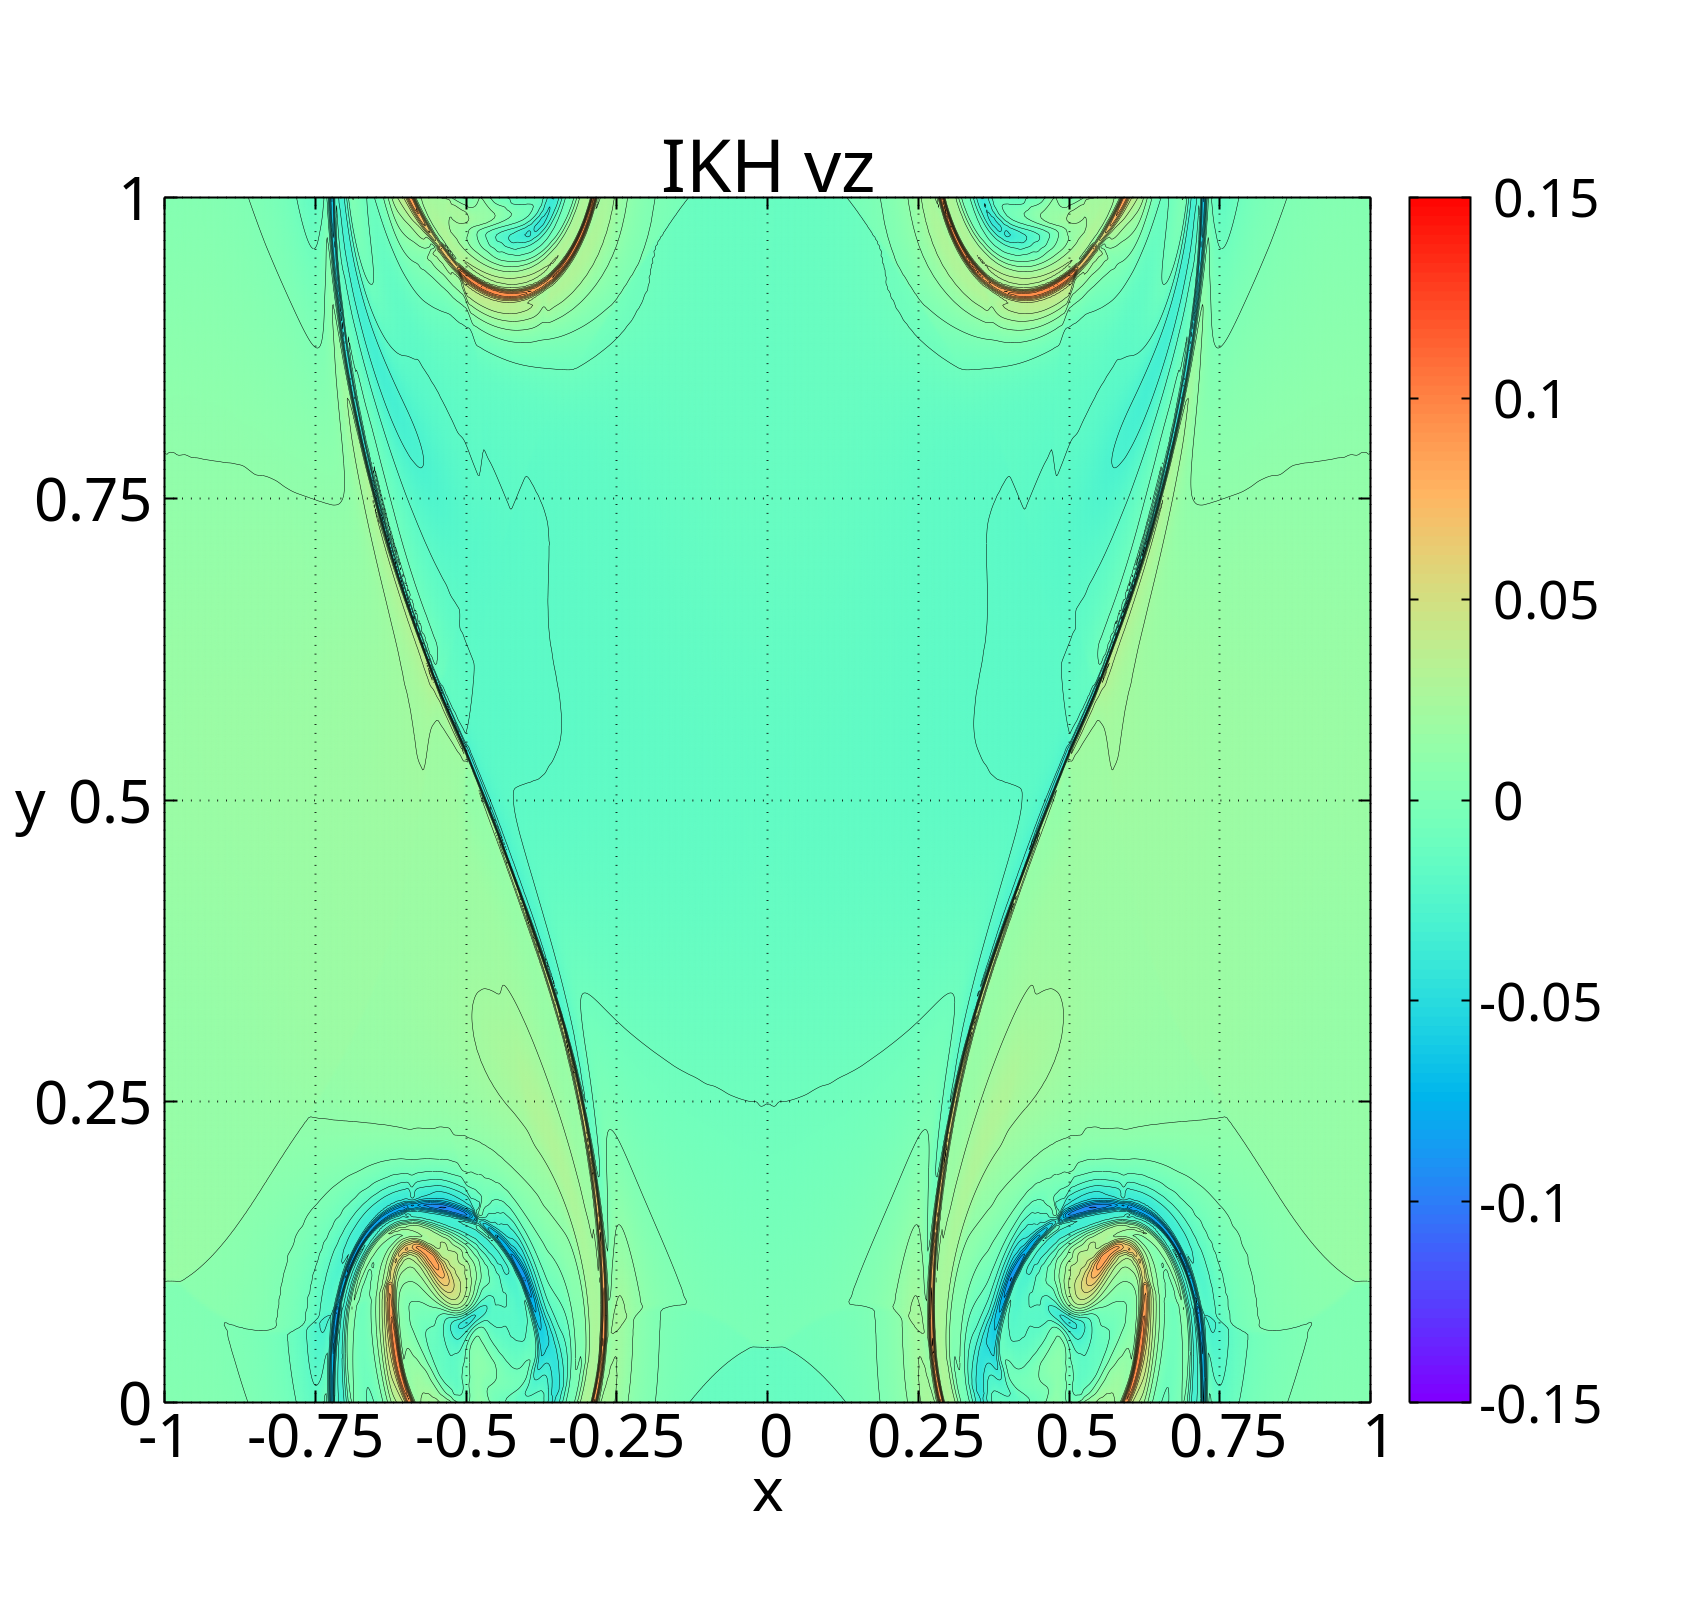
\includegraphics[width=0.24\linewidth]{images/vzs6.png}
    \vspace*{-0.5cm}
    \caption{Velocidad en z para diferentes valores de conductividad}
    \end{figure}
    \hspace{0.2mm}
    \vspace*{-0.5cm}
  \end{minipage} 
  \vspace*{-0.3cm}
}
%%%%%%%%%%%%%%%%%%%%%%%%%%%%%%%%%%%%%%%%%%%%%%%%%%%%%%%%%%%%%%%%%%%%%%%%%%%%%%
  \headerbox{Referencias}{name=references,column=2,above=bottom}{
%%%%%%%%%%%%%%%%%%%%%%%%%%%%%%%%%%%%%%%%%%%%%%%%%%%%%%%%%%%%%%%%%%%%%%%%%%%%%%
%%%%%%%%%%%%%%%%%%%%%%%%%%%%%%%%%%%%%%%%%%%%%%%%%%%%%%%%%%%%%%%%%%%%%%%%%%%%%%

    \smaller
    \bibliographystyle{ieee}
    \renewcommand{\section}[2]{\vskip 0.05em}
      \begin{thebibliography}{1}\itemsep=-0.01em
        \setlength{\baselineskip}{0.4em}
      \bibitem{1} Chow A., et al., $2023$, ApJL, $951$
      \bibitem{2} Dedner A., et al., $2002$, J. Comput. Phys., $175$, 645 
      \bibitem{3} Miranda S., et al., $2014$, ASP Conf. Series, $488$, 249
      \bibitem{4} Miranda S., et al., $2018$, MNRAS, $476$, 3837
      \bibitem{5} Osmanov, et al., $2008$, A\&A, $490$
      \bibitem{6} Palenzuela, C., Lehner, L., Reula, O., Rezzolla, L., $2009$, MNRAS, $394$
      \bibitem{7} Pimentel O. M., Lora-Clavijo F. D., $2019$, MNRAS, $490$
      \end{thebibliography}
  }
  
%%%%%%%%%%%%%%%%%%%%%%%%%%%%%%%%%%%%%%%%%%%%%%%%%%%%%%%%%%%%%%%%%%%%%%%%%%%%%%
  \headerbox{Set-up}{name=set up,column=1,below=results}{
%%%%%%%%%%%%%%%%%%%%%%%%%%%%%%%%%%%%%%%%%%%%%%%%%%%%%%%%%%%%%%%%%%%%%%%%%%%%%%

    %\begin{minipage}{0.25\linewidth}
    \vspace*{-0.5cm}
         {\small
           \begin{align*}
            \vspace*{-0.8cm}
             \small \Gamma        &= 4/3 \\
            \vspace*{-0.8cm} 
             \small v_y&= A_0 v_{sh}\sin({2\pi x})\exp[-(\frac{y-0.5}{\alpha})^2] \ \ \ \text{si y}   > \text{0.0} \\ 
            \vspace*{-0.8cm}
             \small v_y&=-A_0 v_{sh}\sin({2\pi x})\exp[-(\frac{y+0.5}{\alpha})^2] \ \text{si y}  \leq \text{0.0}  \\
            \vspace*{-0.8cm}
             \small v_x&=v_{sh}\tanh{(\frac{y-0.5}{a})}\ \ \ \ \ \text{si y}  > \text{0.0} \\ 
            \vspace*{-0.8cm} 
             \small v_x&=-v_{sh}\tanh{(\frac{y+0.5}{a})} \ \ \ \ \text{si y}  \leq \text{0.0}\\
            \vspace*{-0.8cm}
             \small (B&_x, B_y, B_z)=(\sqrt{2\mu_p p}, 0, \sqrt{2\mu_t p})\\
           \end{align*}
         }

    \vspace*{-0.8cm}
  %\end{minipage}
   
   %\small $v_x= \left\{ \begin{array}{lcc} v_{sh}\tanh{(\frac{y-0.5}{a})} & si & y > 0.0 \\ \\ -v_{sh}\tanh{(\frac{y+0.5}{a})} & si & y \leq 0.0 \end{array} \right.$\\

    %\small $(B_x, B_y, B_z)=(\sqrt{2\mu_p p}, 0, \sqrt{2\mu_t p})$\\
    
    %\small $v_y= \left\{ \begin{array}{lcc} A_0 v_{sh}\sin({2\pi x})\exp[-(\frac{y-0.5}{\alpha})^2] & si & y > 0.0 \\ \\ -A_0 v_{sh}\sin({2\pi x})\exp[-(\frac{y+0.5}{\alpha})^2] & si & y \leq 0.0 \end{array} \right.$\\

}

%%%%%%%%%%%%%%%%%%%%%%%%%%%%%%%%%%%%%%%%%%%%%%%%%%%%%%%%%%%%%%%%%%%%%%%%%%%%%%
  \headerbox{Campo magnético}{name=background model,column=2,below=results}{
%%%%%%%%%%%%%%%%%%%%%%%%%%%%%%%%%%%%%%%%%%%%%%%%%%%%%%%%%%%%%%%%%%%%%%%%%%%%%%
   \vspace*{-0.3cm}
   \begin{figure}[H]
    \centering
    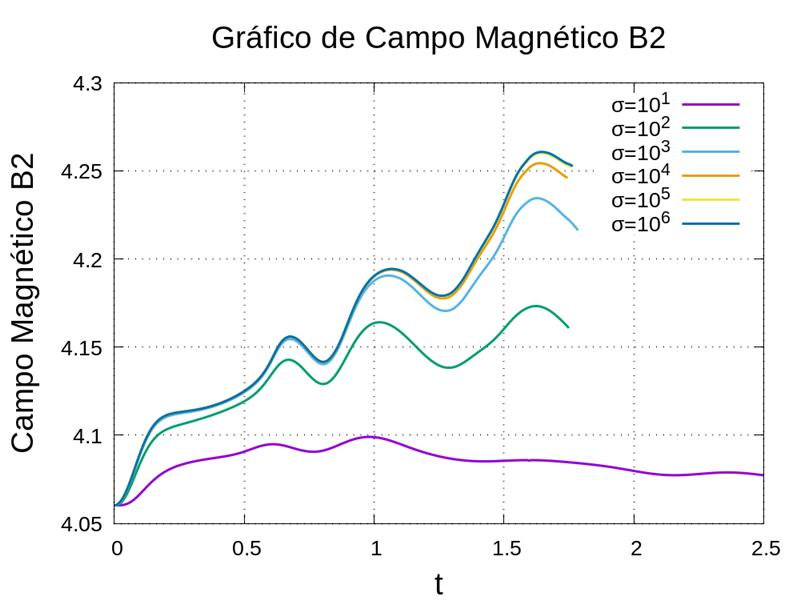
\includegraphics[width=0.49\linewidth]{images/B2.jpg}
    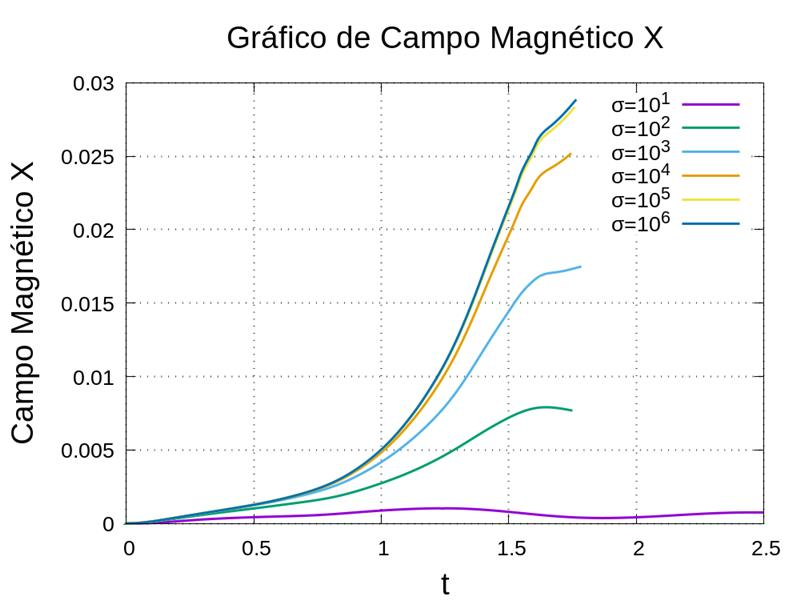
\includegraphics[width=0.49\linewidth]{images/Bx.jpg}
   \end{figure}
   \vspace*{-0.7cm}
   \begin{figure}[H]
    \centering
    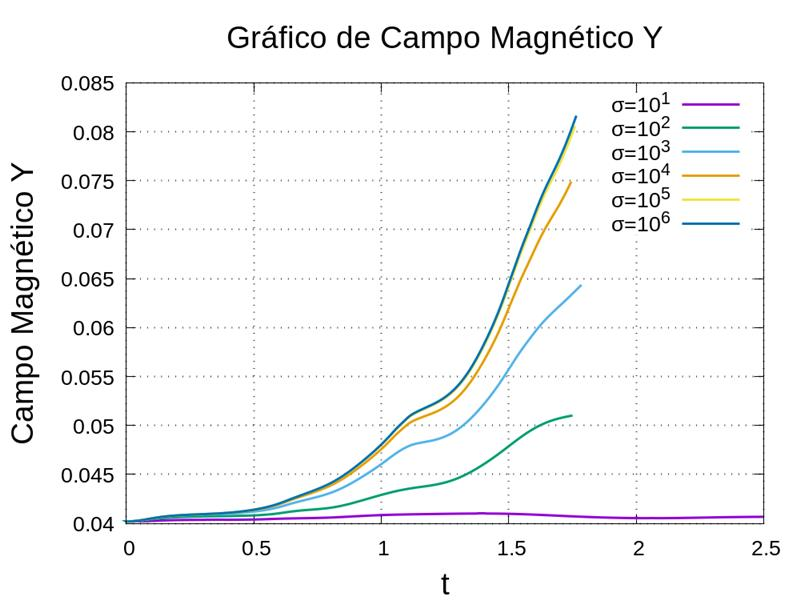
\includegraphics[width=0.49\linewidth]{images/By.jpg}
    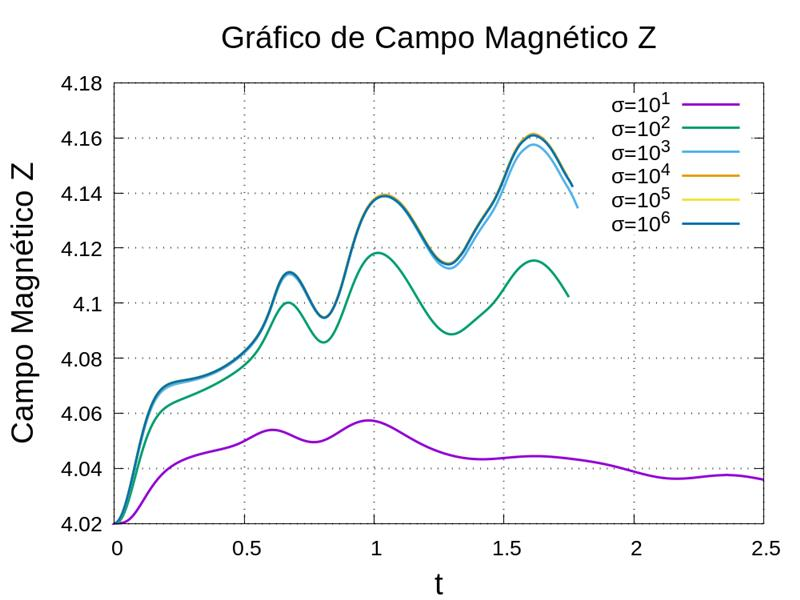
\includegraphics[width=0.49\linewidth]{images/Bz.jpg}
   \end{figure}
   \vspace*{-0.2cm}
}
%%%%%%%%%%%%%%%%%%%%%%%%%%%%%%%%%%%%%%%%%%%%%%%%%%%%%%%%%%%%%%%%%%%%%%%%%%%%%%
\headerbox{{Energía}}{name=speed,column=1,row=0,below=set up, above=bottom}{
  %%%%%%%%%%%%%%%%%%%%%%%%%%%%%%%%%%%%%%%%%%%%%%%%%%%%%%%%%%%%%%%%%%%%%%%%%%%%%%
    \vspace*{-0.5cm}
    \begin{figure}[H]
    \centering
    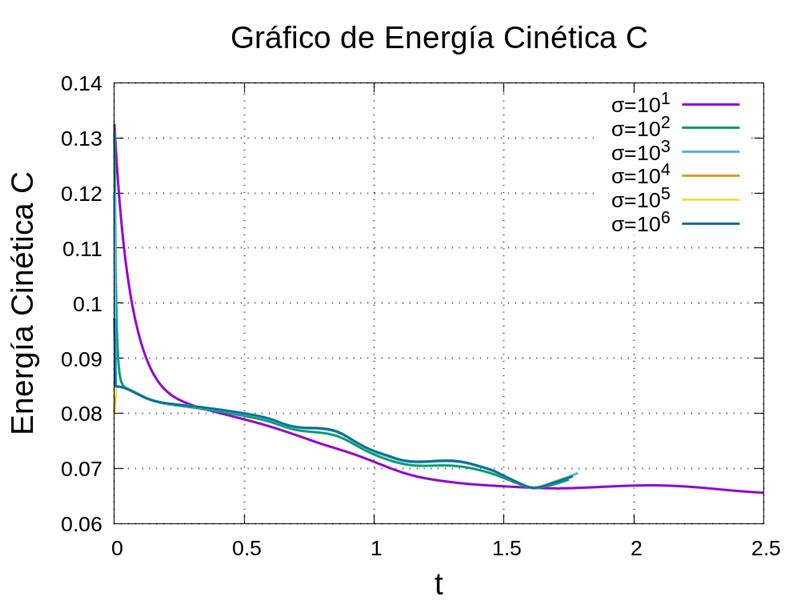
\includegraphics[width=0.49\linewidth]{images/Energía cinética.jpg}
    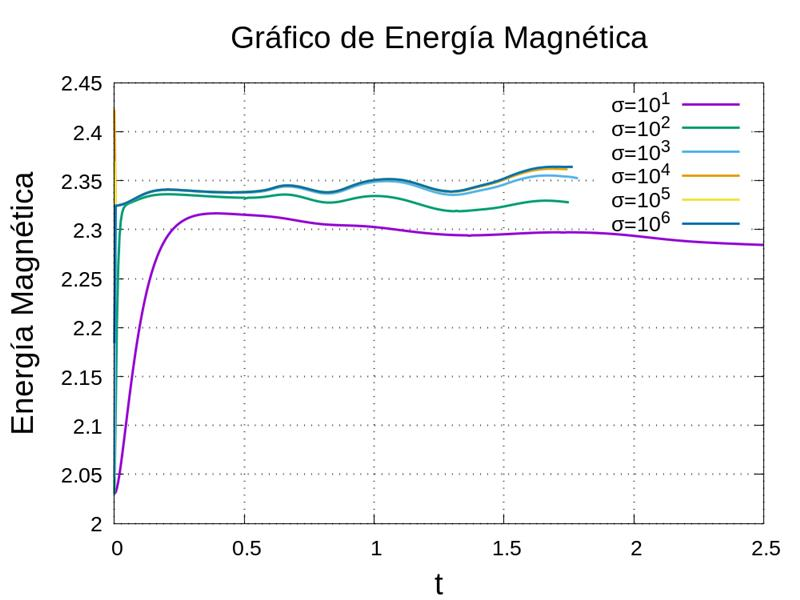
\includegraphics[width=0.49\linewidth]{images/Energía magnética.jpg}
    \end{figure}
    \vspace*{-0.3cm}
    \small{\textbf{Anexos:}
           \begin{figure}[H]
            \vspace*{-0.5cm}
            \centering
            
\includegraphics[width=0.25\linewidth]{images/qr.jpg}
           \end{figure}}
}

%%%%%%%%%%%%%%%%%%%%%%%%%%%%%%%%%%%%%%%%%%%%%%%%%%%%%%%%%%%%%%%%%%%%%%%%%%%%%%
  \headerbox{ecuaciones de la rrmhd}{name=method,column=0,below=problem}{
%%%%%%%%%%%%%%%%%%%%%%%%%%%%%%%%%%%%%%%%%%%%%%%%%%%%%%%%%%%%%%%%%%%%%%%%%%%%%%
    \begin{multicols}{2}
      \vspace*{-3.2cm}
      \hspace*{-2.7cm}
      \begin{minipage}[c][10cm][c]{10cm}
        {\large
          \begin{eqnarray*}
            \partial_t \psi & = & - \nabla \cdot \mathbf{E} \ \ + q - \kappa \psi \\
            \partial_t \phi & = &   - \nabla \cdot \mathbf{B} \ \ - \kappa \phi \\ 
            \partial_t \mathbf{E} & = & \ \ \  \nabla \times \mathbf{B} - \nabla \psi - \mathbf{J} \\
            \partial_t \mathbf{B} & = & - \nabla \times \mathbf{E} - \nabla \phi \\
            \partial_t q & = & - \nabla \cdot \mathbf{J} \\
            \partial_t D &= & - \nabla \cdot \mathbf{F}_D \\ 
            \partial_t {\cal E} &= & - \nabla \cdot \mathbf{F}_{{\cal E}}  \\
            \partial_t \mathbf{S} &= &  - \nabla \cdot \boldsymbol{\mathsf{F}}_{\mathbf{S}} 
        \end{eqnarray*} }
      \end{minipage}
    \end{multicols}
    \vspace*{-2.6cm}
    \noindent  Utilizamos el \emph{sistema aumentado de las ecuaciones de Maxwell} propuesto por Dedner et al \cite{2}. Donde se introducen las nuevas variables (pseudo-potenciales) $\psi$ y $\phi$, que evolucionan de forma similar a $\nabla \cdot \mathbf{B}$ ó $(\nabla \cdot \mathbf{E} \ \ + q)$. Donde $q$ es la densidad de carga y las densidades de masa $D$, de energía ${\cal E}$ y de momentum $\mathbf{S}$, estan dadas por,
    \vspace*{-0.3cm}
    \begin{align*}
      D &= \rho W,  \\
      {\cal E}    &= {\cal E}_{\rm em} + {\cal E}_{\rm hyd} = \frac{1}{2} (\mathbf{E}^2 + \mathbf{B}^2) + \rho h W^2 - p, \\
      \mathbf{S}  &= \mathbf{S}_{\rm em} + \mathbf{S}_{\rm hyd} = \mathbf{E} \times \mathbf{B} + \rho h W^2 \mathbf{v}. 
    \end{align*}
    $W = (1-\mathbf{v}^2)^{-1/2}$ el factor de lorentz y $h$ la entalpía.
    
  }
%%%%%%%%%%%%%%%%%%%%%%%%%%%%%%%%%%%%%%%%%%%%%%%%%%%%%%%%%%%%%%%%%%%%%%%%%%%%%%
  \headerbox{Conclusiones}{name=source,column=0,below=method,above=bottom}{
%%%%%%%%%%%%%%%%%%%%%%%%%%%%%%%%%%%%%%%%%%%%%%%%%%%%%%%%%%%%%%%%%%%%%%%%%%%%%%

    \noindent {\small En resumen, la resistividad en plasmas magnetizados reduce la capacidad del campo magnético para deformarse y amplificar las perturbaciones iniciales. En entornos con alta resistividad, el crecimiento de la inestabilidad es lento y menos efectivo, y la formación de estructuras turbulentas se ven favorecidas.} \\[0.3em]

  }
%
\end{poster}

\end{document}

